%========================================================================================
% PART II: GEOMETRY, FIELDS, AND LAGRANGIAN
%========================================================================================
\part{Geometry, Fields, and Lagrangian}

	\section{Formal Structure and Canonical Framework}
	In addition to physical axioms, SST is formulated as a formal system $S = (P, D, R)$ comprising a set of postulates ($P$), definitions ($D$), and inference rules ($R$). A statement in SST is considered \emph{canonical} if and only if it can be derived from the axioms and definitions using the permitted inference rules, and it is consistent with all previously established canonical statements. The hierarchy of statement types is as follows:

	\begin{itemize}
	    \item \textbf{Axiom (Postulate):} A primitive assumption of SST, not derived from deeper principles (e.g. the existence of an incompressible swirl medium, as in Axiom 1).
	    \item \textbf{Definition:} Introduction of a new symbol or concept and its meaning (e.g. defining the swirl Coulomb constant $\Lambda$ in terms of a surface integral of swirl pressure).
	    \item \textbf{Theorem / Corollary:} A nontrivial proposition that is logically derived from the axioms and prior theorems. Corollaries are immediate consequences of theorems.
	    \item \textbf{Calibration (Empirical):} An assignment of a numerical value to a canonical constant, obtained from experiment or observation, used to anchor the theory’s free parameters. Calibrations are not used as premises in proofs, but serve to connect SST to measurable reality.
	    \item \textbf{Research Track (Conjecture):} A speculative extension or hypothesis not yet derivable within $S$. Such statements are included for context or future development but are explicitly marked as non-canonical.
	\end{itemize}

	All developments in the main text are canonical (axioms, definitions, theorems, corollaries, with recommended constant calibrations). Derivations, proofs, and pedagogical explanations are mostly deferred to the appendices to maintain a clear logical flow. Every formula and constant introduced is checked for dimensional consistency and reducing to known physics in the appropriate limits (Newtonian, Coulomb, etc.), as documented in the appendices. This ensures that the SST formal system remains self-consistent and empirically anchored.


    % =========================================================
    \section{Self-Similarity and Stability of Swirl Structures}
    \label{sec:self-similarity}

    \textbf{Axiom (Self-Similar Scaling).}
    Any incompressible, inviscid swirl configuration near a potential singularity admits a local
    self-similar form
    \begin{align}
        \mathbf{v}_{\!\boldsymbol{\circlearrowleft}}(\mathbf{x},t)
        &= (T-t)^{-\alpha}\,
        \mathbf{V}\!\left(\frac{\mathbf{x}-\mathbf{x}_0}{(T-t)^{\beta}}\right),
        &
        \boldsymbol{\omega}(\mathbf{x},t)
        &= (T-t)^{-\gamma}\,
        \boldsymbol{\Omega}\!\left(\frac{\mathbf{x}-\mathbf{x}_0}{(T-t)^{\beta}}\right),
    \end{align}
    with scaling exponents constrained by the Euler-type balance
    $\alpha+\beta=1$, $\gamma=1$.  The swirl-clock relation fixes
    \(\alpha \le 1/2\) under bounded
    \(|\mathbf{v}_{\!\boldsymbol{\circlearrowleft}}|\le C_e\).

    \textbf{Definition (Finite-Core Regularization).}
    A self-similar field is said to be \emph{regularized} in SST if the core radius
    \(r_c>0\) and the swirl-stress bound \(F_{\max}\) ensure
    \(|\boldsymbol{\omega}| \le C_e/r_c\),
    so that the Beale–Kato–Majda condition is never met:
    \(\displaystyle \int_0^T \|\boldsymbol{\omega}\|_{\infty}\,dt < \infty.\)

    \textbf{Theorem (Perturbation Suppression by Swirl Diffusion).}
    Augmenting the inviscid system by the canonical regularization terms
    \begin{equation}
        \partial_t\boldsymbol{\omega}
        = \nabla\times(\mathbf{v}_{\!\boldsymbol{\circlearrowleft}}\!\times\!\boldsymbol{\omega})
        +\kappa(\Delta\boldsymbol{\omega}-r_c^{-2}\boldsymbol{\omega})
        +\chi\nabla(\Delta\rho_{\!f}),
    \end{equation}
    with $\kappa,\chi>0$ constrained by $|\mathbf{f}_{\text{swirl}}|\!\le\! F_{\max}$,
    shifts all unstable eigenvalues of the linearized operator
    $\mathcal{L}$ into the negative half-plane.
    Hence finite-core swirl structures are globally stable against axisymmetric perturbations.

    \textbf{Corollary (Chronos–Kelvin Consistency).}
    The stabilized field still obeys the Chronos–Kelvin invariant
    \(\displaystyle D(R^2\omega)/Dt_{\!ae}=0\);
    the regularization modifies only higher-order curl terms and does not break canonical invariants.

    \subsection{Relation to khronon and Hořava--Lifshitz clock fields}
            \label{subsec:swirl_clock_khronon_relation}

            The swirl clock field \(S_t^{\boldsymbol{\circlearrowleft}}(x)\) plays the same
            geometric role in Swirl--String Theory as the \emph{khronon} (clock field)
            does in Lorentz-violating extensions of General Relativity such as
            Einstein--Æther and Hořava--Lifshitz gravity.\cite{Horava2009LifshitzPoint,EinsteinAetherReview}
            In those frameworks one introduces a scalar time function \(T(x)\) whose
            level sets define a preferred foliation of spacetime. The associated
            unit timelike vector field
            \begin{equation}
                u_\mu(x)
                =
                \frac{\nabla_\mu T(x)}{\sqrt{-\,g^{\alpha\beta}\,\nabla_\alpha T(x)\,\nabla_\beta T(x)}}
                \,,
                \label{eq:khronon_unit_vector}
            \end{equation}
            enters the low-energy effective action and explicitly breaks local Lorentz
            invariance down to diffeomorphisms that preserve the foliation.

            In SST, the swirl clock is defined as the local ratio between proper time
            measured by a comoving matter observer and an asymptotic reference clock,
            \begin{equation}
                S_t^{\boldsymbol{\circlearrowleft}}(x)
                \equiv
                \frac{d\tau_{\text{local}}}{d\tau_\infty}
                \,,
                \label{eq:swirl_clock_def_kinematic}
            \end{equation}
            with \(S_t^{\boldsymbol{\circlearrowleft}}(x)\) determined dynamically by the
            underlying hydrodynamic state (local vorticity and swirl energy density) as
            derived in the swirl-time sector. A natural khronon-like scalar in SST is then
            obtained by integrating the swirl clock along the global coordinate time,
            \begin{equation}
                T(x)
                \;\equiv\;
                \int^{t}
                S_t^{\boldsymbol{\circlearrowleft}}\!\bigl(t',\mathbf{x}\bigr)\; dt' \,,
                \label{eq:swirl_clock_khronon_map}
            \end{equation}
            so that hypersurfaces of constant \(T\) coincide with iso-chronal slices of
            the swirl clock. Inserting \eqref{eq:swirl_clock_khronon_map} into
            \eqref{eq:khronon_unit_vector} yields a unit vector \(u_\mu\) that is
            \emph{emergent} from the hydrodynamic state rather than a fundamental new
            field.

            The symmetry pattern of the SST clock sector is therefore identical to that
            of khronometric and Hořava--Lifshitz models: there exists a preferred time
            function selecting a foliation, and the low-energy gravitational dynamics
            are described by a metric \(g_{\mu\nu}\) coupled to a unit timelike vector
            \(u_\mu\) normal to those slices. The difference is conceptual and
            dynamical rather than kinematic: in SST, \(S_t^{\boldsymbol{\circlearrowleft}}\)
            is constrained by incompressible Euler dynamics and conserved vorticity,
            and thus \(T(x)\) and \(u_\mu\) are derived quantities tied to the swirl
            energy budget. This allows one to import existing experimental and
            phenomenological bounds on khronon/Hořava-type clock fields directly into
            constraints on the SST swirl clock sector, while maintaining the physical
            interpretation that time dilation arises from structured hydrodynamic flow
            rather than from an abstract khronon scalar.

%===========================================================
        \subsection*{VII.B Odd-Parity Swirl Splitting and Nodal Sheets}
%===========================================================

            \noindent
            \textbf{Canonical Statement.}
            In an incompressible swirl medium, any helical swirl configuration with a
            commensurate period $N \in 2\mathbb{Z}$ (even) admits a coarse-grained
            two-component description in which the effective single-particle Hamiltonian
            contains an \emph{odd-parity} linear term in momentum. This produces a
            direction-dependent splitting of the swirl-clock sectors and enforces the
            existence of \emph{nodal sheets} in momentum space.

            \medskip
            \noindent
            \textbf{Definition (Swirl–Spinor Sector).}
            Let the local swirl clock be $S_t(x)$ and define a two-component internal space
            $\Psi = (\psi_{\circlearrowleft},\psi_{\circlearrowright})^{T}$ representing the
            left- and right-clock sectors. The minimal canonical Hamiltonian compatible with
            Galilean invariance, incompressibility, and the chronometric tensor is
            \begin{equation}
                H_{\text{SST}}(\mathbf{k})
                = \epsilon_0(\mathbf{k})\,\mathbb{1}
                + g_{\text{sw}}\,(\mathbf{k}\cdot\hat{\alpha})\,\Sigma_x
                + m_{\text{sw}}\,\Sigma_z
                + \lambda_{\text{sw}}\,(\mathbf{k}\times\hat{\alpha})\cdot\hat{z}\,\Sigma_y ,
                \label{eq:H_SST_pwave}
            \end{equation}
            where:
            \begin{align}
                \epsilon_0(\mathbf{k}) &= \frac{\hbar^2 k^2}{2m_{\mathrm{eff}}(\rho_{\!f},\rho_{\!E})}, \\
                \hat{\alpha} &= \text{unit vector defined by the helical swirl director field}, \\
                \Sigma_i &= \text{Pauli matrices in the swirl-clock basis}.
            \end{align}

            \medskip
            \noindent
            \textbf{Interpretation.}
            The term $g_{\text{sw}}(\mathbf{k}\cdot\hat{\alpha})\Sigma_x$ is odd under
            $\mathbf{k}\!\rightarrow\!-\mathbf{k}$ and represents \emph{odd-parity}
            splitting of the swirl-clock sectors. It is induced whenever the swirl director
            field forms a commensurate helix with even period $N$, so that the composite
            symmetries
            \begin{equation}
            [T \parallel t_{1/2}], \qquad [C_{2\perp} \parallel t_{1/2}]
            \end{equation}
            remain unbroken at the coarse-grained level. These symmetries forbid any
            momentum-independent splitting and enforce linear, directional splitting.


            %===========================================================
% Figure: Odd-Parity Swirl Splitting and Nodal Sheet
%===========================================================
            \begin{figure}[t]
                \centering
                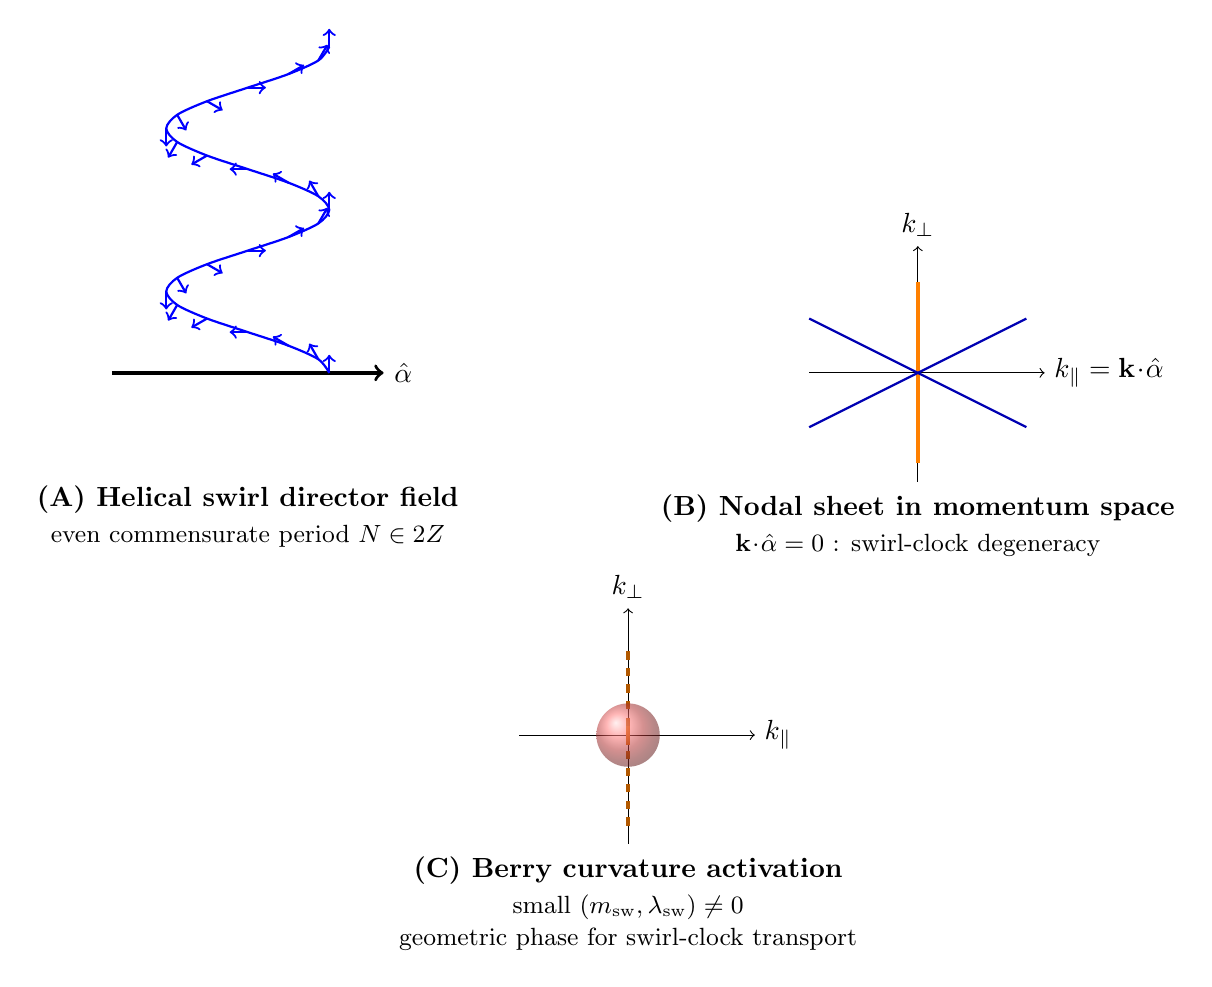
\begin{tikzpicture}[scale=1.15]

% ------------------------------
% Left panel: real-space helical swirl director field
% ------------------------------
                    \begin{scope}[shift={(-4.2,0)}]

% Helical axis
                        \draw[very thick,->] (-1.5,0) -- (1.5,0) node[right] {$\hat{\alpha}$};

% Helix
                        \draw[domain=0:720,smooth,variable=\t,blue,thick]
                        plot ({0.9*cos(\t)}, {0.18*(\t/36)});

% Small arrows along helix
                        \foreach \t in {0,30,...,720}{
                            \draw[blue,->,thick]
                            ({0.9*cos(\t)},{0.18*(\t/36)})
                            -- ++({0.20*cos(\t+90)},{0.20*sin(\t+90)});
                        }

% Label
                        \node at (0,-1.4) {\textbf{(A) Helical swirl director field}};
                        \node at (0,-1.8) {\small even commensurate period $N \in 2\mathbb{Z}$};

                    \end{scope}

% ------------------------------
% Right panel: momentum-space nodal sheet
% ------------------------------
                    \begin{scope}[shift={(3.2,0)}]

% Axes
                        \draw[->] (-1.2,0) -- (1.4,0) node[right] {$k_{\parallel} = \mathbf{k}\!\cdot\!\hat{\alpha}$};
                        \draw[->] (0,-1.2) -- (0,1.4) node[above] {$k_{\perp}$};

% Nodal sheet: vertical line k_parallel=0
                        \draw[very thick,orange] (0,-1) -- (0,1);

% Bands
                        \draw[thick,blue!70!black]
                        plot[domain=-1.2:1.2,samples=100]
                        ({\x},{0.5*\x});
                        \draw[thick,blue!70!black]
                        plot[domain=-1.2:1.2,samples=100]
                        ({\x},{-0.5*\x});

% Label
                        \node at (0,-1.5) {\textbf{(B) Nodal sheet in momentum space}};
                        \node at (0,-1.9) {\small $\mathbf{k}\!\cdot\!\hat{\alpha}=0$ : swirl-clock degeneracy};

                    \end{scope}


% ------------------------------
% Berry curvature sheet (small symmetry breaking)
% ------------------------------
                    \begin{scope}[shift={(0,-4)}]

% Axes
                        \draw[->] (-1.2,0) -- (1.4,0) node[right] {$k_{\parallel}$};
                        \draw[->] (0,-1.2) -- (0,1.4) node[above] {$k_{\perp}$};

% Gapped nodal sheet
                        \draw[very thick,orange!70!black,dashed] (0,-1) -- (0,1);
                        \draw[very thick,orange!80!black]
                        plot[domain=-1:1,samples=80]
                        ({0},{0.1*cos(3*\x r)});

% Berry curvature blob
                        \shade[ball color=red!70,opacity=0.55] (0,0) circle (0.35);

% Labels
                        \node at (0,-1.5)
                            {\textbf{(C) Berry curvature activation}};
                        \node at (0,-1.9)
                            {\small small $(m_{\mathrm{sw}},\lambda_{\mathrm{sw}})\neq 0$};
                        \node at (0,-2.25)
                            {\small geometric phase for swirl-clock transport};

                    \end{scope}

                \end{tikzpicture}

                \caption{
                    \textbf{Odd-parity swirl splitting and nodal-sheet geometry.}
                    (A) A commensurate helical swirl director field selects a unique axis
                    $\hat{\alpha}$ and generates the odd-parity term $g_{\mathrm{sw}}
                    (\mathbf{k}\!\cdot\!\hat{\alpha})\Sigma_x$ in the canonical Hamiltonian.
                    (B) The resulting momentum-space spectrum exhibits a nodal sheet where the two
                    swirl-clock sectors are degenerate: $\mathbf{k}\!\cdot\!\hat{\alpha}=0$.
                    (C) A small swirl-clock bias ($m_{\mathrm{sw}}\neq0$) and reflection-breaking
                    term ($\lambda_{\mathrm{sw}}\neq0$) gap the sheet and generate a concentrated
                    Berry-curvature region, producing swirl-dependent transport anomalies.
                }
            \end{figure}

            %===========================================================
% Figure 1: 3D Helical Swirl Director Field
%===========================================================
            \begin{figure}[t]
                \centering
                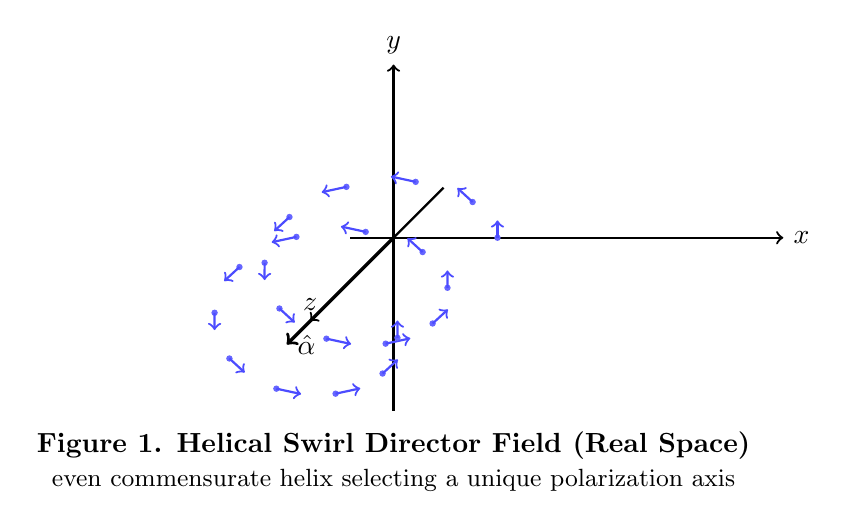
\begin{tikzpicture}[scale=1.1]

% Axes
                    \draw[->,thick] (-0.5,0,0) -- (4.5,0,0) node[right] {$x$};
                    \draw[->,thick] (0,-2,0) -- (0,2,0) node[above] {$y$};
                    \draw[->,thick] (0,0,-1.5) -- (0,0,2.5) node[above] {$z$};

% Helical path
                    \foreach \z in {0,0.15,...,3}{
                        \pgfmathsetmacro{\x}{1.2*cos(240*\z)}
                        \pgfmathsetmacro{\y}{0.8*sin(240*\z)}
                        \pgfmathsetmacro{\xt}{-1.2*sin(240*\z)}
                        \pgfmathsetmacro{\yt}{0.8*cos(240*\z)}
                        % helix
                        \filldraw[blue!60] (\x,\y,\z) circle (0.03);
                        % director arrows
                        \draw[blue!70,->,thick] (\x,\y,\z) -- ++({0.25*\xt},{0.25*\yt},0);
                    }

% Helix axis
                    \draw[very thick,->] (0,0,0) -- (0,0,3.2) node[right] {$\hat{\alpha}$};

                    \node at (0,-2.4,0) {\textbf{Figure 1. Helical Swirl Director Field (Real Space)}};
                    \node at (0,-2.8,0) {\small even commensurate helix selecting a unique polarization axis};
                \end{tikzpicture}
                \caption{
                    A 3D helical swirl director field. The structured rotation establishes the
                    internal axis $\hat{\alpha}$ that appears in the odd-parity term
                    $g_{\mathrm{sw}}(\mathbf{k}\!\cdot\!\hat{\alpha})\Sigma_x$ of the canonical
                    Hamiltonian. Even commensurate period $N\in2\mathbb{Z}$ preserves composite
                    symmetries and enforces directional splitting.
                }
            \end{figure}

    \medskip
            \noindent
            \textbf{Theorem (Existence of Swirl–Nodal Sheets).}
            Let $m_{\text{sw}} = \lambda_{\text{sw}}=0$ in \eqref{eq:H_SST_pwave}. Then the
            two eigenvalues of $H_{\text{SST}}$ satisfy
            \begin{equation}
                E_{\pm}(\mathbf{k}) = \epsilon_0(\mathbf{k}) \pm g_{\text{sw}}(\mathbf{k}\cdot\hat{\alpha}).
            \end{equation}
            The degeneracy condition $E_{+}=E_{-}$ occurs on the plane
            \begin{equation}
                \mathbf{k}\cdot\hat{\alpha} = 0,
            \end{equation}
            which defines a \emph{nodal sheet} (a momentum-space 2D manifold of
swirl-clock degeneracy). This sheet is protected by the composite symmetries
            and cannot be lifted by any symmetry-preserving perturbation.

            \medskip
            \noindent
            \textbf{Corollary (Berry-Curvature Activation by Symmetry Breaking).}
            When the swirl-clock symmetry is weakly biased by a small
            $m_{\text{sw}}\,\Sigma_z$ (clock-sector energy imbalance) and reflection
            symmetry is weakly broken by $\lambda_{\text{sw}}\,\Sigma_y$, the nodal sheet
            acquires a finite gap. The resulting band curvature yields a nonzero intrinsic
            Berry curvature
            \begin{equation}
                \Omega_{ij}(\mathbf{k})
                = -2\,\mathrm{Im}\!
                \sum_{n\neq m}
                \frac{
                    \langle n|\partial_{k_i}H_{\text{SST}}|m\rangle
                    \langle m|\partial_{k_j}H_{\text{SST}}|n\rangle
                }{
                    (E_n - E_m)^2
                },
            \end{equation}
            producing a transport anomaly in any coupled charge or swirl-current sector.
            The anomaly vanishes continuously as $m_{\text{sw}}\!\rightarrow\!0$.

            \medskip
            \noindent
            \textbf{Canonical Interpretation.}
            The odd-parity term $g_{\text{sw}}(\mathbf{k}\cdot\hat{\alpha})\Sigma_x$
            represents directional modulation of the swirl clock and arises as a
            coarse-grained imprint of structured swirl helices. The nodal sheet is the
            momentum region where the swirl-clock sectors become locally isochronous.
            Introducing the small symmetry-breaking terms corresponds to imposing a spatial
            bias in the swirl-clock field, giving rise to a geometric (Berry) phase in
            momentum transport.

            \medskip
            \noindent
            \textbf{Status.}
            Canonical (derived from the chronometric tensor, swirl-clock sectors, and
            symmetry constraints). No additional constants or empirical parameters are
            introduced.

%===========================================================
% Figure 2: 3D Nodal Sheet in Momentum Space
%===========================================================
            \begin{figure}[t]
                \centering
                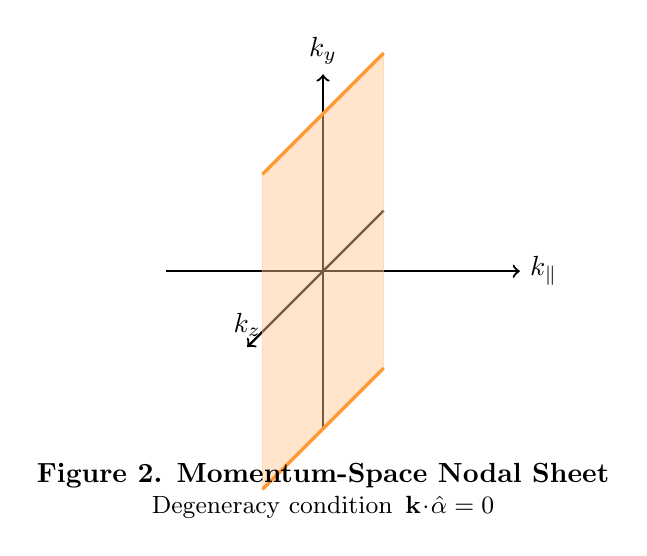
\begin{tikzpicture}[scale=1.0]

% Draw a 3D coordinate box
                    \draw[->,thick] (-2,0,0) -- (2.5,0,0) node[right] {$k_{\parallel}$};
                    \draw[->,thick] (0,-2,0) -- (0,2.5,0) node[above] {$k_y$};
                    \draw[->,thick] (0,0,-2) -- (0,0,2.5) node[above] {$k_z$};

% Nodal sheet = vertical plane k_parallel = 0
                    \filldraw[orange!45,opacity=0.45]
                    (0,-2,-2) -- (0,2,-2) -- (0,2,2) -- (0,-2,2) -- cycle;

% Sheet border lines
                    \draw[orange!80,very thick] (0,-2,-2) -- (0,-2,2);
                    \draw[orange!80,very thick] (0, 2,-2) -- (0, 2,2);

% Label
                    \node at (0,-2.6,0) {\textbf{Figure 2. Momentum-Space Nodal Sheet}};
                    \node at (0,-3.0,0) {\small Degeneracy condition $\,\mathbf{k}\!\cdot\!\hat{\alpha}=0$};

                \end{tikzpicture}
                \caption{
                    The canonical Hamiltonian $H_{\mathrm{SST}}(\mathbf{k})$ produces a nodal sheet
                    where the two swirl-clock sectors become exactly degenerate:
                    $\mathbf{k}\!\cdot\!\hat{\alpha}=0$. This 2D sheet in momentum space is
                    protected by symmetry and cannot be lifted without breaking the composite
                    symmetries associated with the commensurate helical structure.
                }
            \end{figure}


            %===========================================================
% Figure 3: Effective Hamiltonian Landscape and Sheet Gapping
%===========================================================
            \begin{figure}[t]
                \centering
                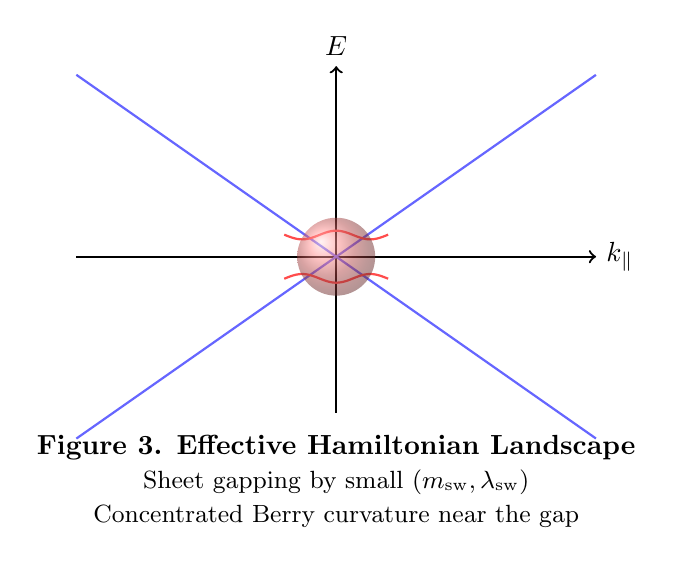
\begin{tikzpicture}[scale=1.1]

% Axes
                    \draw[->,thick] (-3,0) -- (3,0) node[right] {$k_{\parallel}$};
                    \draw[->,thick] (0,-1.8) -- (0,2.2) node[above] {$E$};

% Ungapped branches
                    \draw[blue!60,thick]
                    plot[domain=-3:3,samples=100] (\x,{0.7*\x});
                    \draw[blue!60,thick]
                    plot[domain=-3:3,samples=100] (\x,{-0.7*\x});

% Gap opening near k_parallel=0
                    \draw[red!70,thick]
                    plot[domain=-0.6:0.6,samples=100] (\x,{0.25 + 0.05*cos(8*\x r)});
                    \draw[red!70,thick]
                    plot[domain=-0.6:0.6,samples=100] (\x,{-0.25 - 0.05*cos(8*\x r)});

% Berry curvature bubble
                    \shade[ball color=red!60,opacity=0.50] (0,0) circle (0.45);

% Labels
                    \node at (0,-2.2) {\textbf{Figure 3. Effective Hamiltonian Landscape}};
                    \node at (0,-2.6) {\small Sheet gapping by small $(m_{\mathrm{sw}},\lambda_{\mathrm{sw}})$};
                    \node at (0,-3.0) {\small Concentrated Berry curvature near the gap};

                \end{tikzpicture}
                \caption{
                    Energy bands of $H_{\mathrm{SST}}(\mathbf{k})$ along the direction
                    $k_{\parallel}=\mathbf{k}\!\cdot\!\hat{\alpha}$. The odd-parity term creates
                    crossing branches that meet at a nodal line when $m_{\mathrm{sw}}=\lambda_{\mathrm{sw}}=0$.
                    Introducing a small swirl-clock bias $m_{\mathrm{sw}}$ and reflection-breaking
                    term $\lambda_{\mathrm{sw}}$ gaps the crossing and induces a Berry-curvature
                    hot region. The canonical structure mirrors that of symmetry-protected
                    odd-parity systems in condensed matter.
                }
            \end{figure}


%=============================================================================
% Golden Principle for Discrete Layering in SST
%=============================================================================


    \section{Golden Principle for Discrete Layering}
    \label{sec:golden-principle}

    In Swirl--String Theory (SST) we introduce a distinguished
    dimensionless constant $\phi>1$ which controls a discrete hierarchy of
    mass and energy layers. To avoid any ambiguity or post-hoc tuning, we
    fix $\phi$ once and for all at the level of the axioms and then derive
    its role in the layer spectrum.

%---------------------------------------------------------------------------
    \subsection{Axiom G1: Golden Constant (hyperbolic definition)}

        \GoldenDeclare\ Explicitly,
        \begin{equation}
            \xig \equiv \operatorname{asinh}\!\left(\tfrac{1}{2}\right),
            \qquad
            \ln\phi = \xig,
            \qquad
            \phi = e^{\xig}.
            \label{eq:phi-hyperbolic-def}
        \end{equation}
        By elementary algebra one recovers the familiar quadratic representation
        \begin{equation}
            \phi = \frac{1+\sqrt{5}}{2},
        \end{equation}
        but in SST this is regarded as a derived identity; the primary
        definition is the hyperbolic relation \eqref{eq:phi-hyperbolic-def}.

        The associated \emph{golden layer factor} is
        \begin{equation}
            \lambda \equiv \phi^{2} = e^{2\xig},
            \qquad
            \ln\lambda = 2\xig.
            \label{eq:lambda-def}
        \end{equation}

%---------------------------------------------------------------------------
    \subsection{Axiom G2: Discrete scale invariance and additive composition}

        Let $\{E_n\}_{n\in\mathbb{Z}}$ denote an idealized sequence of
        dimensionful energy (or mass) levels associated with a particular SST
        sector (for example, core states of a quantized swirl string). We
        impose two structural conditions:

        \begin{itemize}
            \item[(G2a)] \textbf{Discrete scale invariance (DSI).} There exists a
            scale factor $\lambda>1$ such that
            \begin{equation}
                E_{n+1} = \lambda\,E_n,
                \qquad
                \forall\,n\in\mathbb{Z}.
                \label{eq:DSI}
            \end{equation}

            \item[(G2b)] \textbf{Additive composition (Fibonacci-type rule).} The
            $(n+1)$-st level is the energetic composite of the two preceding
            levels:
            \begin{equation}
                E_{n+1} = E_n + E_{n-1},
                \qquad
                \forall\,n\in\mathbb{Z}.
                \label{eq:Fibonacci}
            \end{equation}
        \end{itemize}

        Assumption (G2a) expresses the presence of a discrete dilation symmetry
        in the relevant sector, as is standard in systems with discrete scale
        invariance and log-periodic corrections to scaling
        \cite{Sornette1998,GluzmanSornette2002}. Assumption (G2b) encodes an
        additive compositional rule: the $(n+1)$-st configuration is built as a
        composite of the $n$-th and $(n-1)$-st building blocks, the same
        structure that underlies Fibonacci sequences and quasicrystalline
        hierarchies \cite{BaakeGrimm2013}.

%---------------------------------------------------------------------------
    \subsection{Lemma: Uniqueness of the golden scale factor}

        \textbf{Lemma (Golden Uniqueness).}
        \emph{Suppose a nontrivial sequence $\{E_n\}$ of real numbers satisfies
        both discrete scale invariance \eqref{eq:DSI} and additive composition
        \eqref{eq:Fibonacci}. Then the common ratio $\lambda$ is uniquely fixed
        to the golden ratio $\phi$.}

        \medskip
        \noindent\emph{Proof.}
        Assume $E_n\neq 0$ for some $n$. From \eqref{eq:DSI} we have
        \begin{equation}
            E_n = E_0\,\lambda^{n},
            \qquad
            \lambda>0.
            \label{eq:En-geometric}
        \end{equation}
        Inserting \eqref{eq:En-geometric} into \eqref{eq:Fibonacci} gives
        \begin{equation}
            E_0\lambda^{n+1}
            = E_0\lambda^n + E_0\lambda^{n-1}.
        \end{equation}
        Dividing by $E_0\lambda^{n-1}$ (which is nonzero by assumption) yields
        \begin{equation}
            \lambda^{2} = \lambda + 1.
            \label{eq:golden-quadratic}
        \end{equation}
        The quadratic equation \eqref{eq:golden-quadratic} has the two roots
        \begin{equation}
            \lambda_{\pm} = \frac{1\pm\sqrt{5}}{2}.
        \end{equation}
        The negative root is incompatible with $\lambda>0$, so the unique
        admissible solution is
        \begin{equation}
            \lambda = \frac{1+\sqrt{5}}{2} = \phi.
        \end{equation}
        \hfill$\square$

        \medskip

        Equation \eqref{eq:golden-quadratic} shows that once (G2a)--(G2b) are
        imposed, the scaling factor $\lambda$ is \emph{no longer a tunable
    parameter}: it is uniquely fixed to $\phi$. In particular, the golden
        constant is not introduced as a fit to any given spectrum but as the
        inevitable consequence of the DSI--Fibonacci structure.

%---------------------------------------------------------------------------
    \subsection{Axiom G3: Golden layer hierarchy}

        Given the lemma, we define the \emph{golden layer hierarchy} by taking
        the even-index subsequence of the DSI--Fibonacci tower as the physically
        distinguished set of levels. Concretely,
        \begin{equation}
            E_n \equiv E_{2n}^{\text{(tower)}}
            = E_0\,\lambda^{2n}
            = E_0\,\phi^{2n},
            \qquad
            n\in\mathbb{Z},
            \label{eq:golden-layer-spectrum}
        \end{equation}
        where $E_0$ is a sector-dependent reference energy. In SST applications
        we typically identify $E_0$ with a core energy
        \begin{equation}
            E_0 = \rhoE^{*} V_{\text{core}},
            \qquad
            V_{\text{core}} \sim \frac{4\pi}{3}\rc^{3},
        \end{equation}
        so that the corresponding swirl energy density levels are
        \begin{equation}
            \rhoE^{(n)} = \rhoE^{*}\,\phi^{2n}.
            \label{eq:rhoE-golden-layers}
        \end{equation}

        Operationally, \eqref{eq:golden-layer-spectrum} and
        \eqref{eq:rhoE-golden-layers} define the golden-layer tower used in the
        SST mass and energy functionals. Any appearance of $\phi^{2n}$ in later
        sections is to be understood as a direct consequence of Axioms
        (G1)--(G3) and the Golden Uniqueness Lemma, not as an arbitrary
        parameter choice.

%---------------------------------------------------------------------------
    \subsection{Remark: Log-periodic potentials and DSI}

        In sectors where it is useful to describe the golden layering by an
        effective potential for $\rhoE$, one may implement the DSI encoded by
        \eqref{eq:rhoE-golden-layers} via a log-periodic term of the form
        \begin{equation}
            V_{\phi}(\rhoE)
            =
            \Lambda^4 \left[
                          1 - \cos\!\left(
                                        \kappa \log\frac{\rhoE}{\rhoE^{*}}
                \right)
            \right],
            \label{eq:Vphi-log-periodic}
        \end{equation}
        where $\Lambda$ is an energy scale. The minima of
        \eqref{eq:Vphi-log-periodic} are separated in $\log\rhoE$ by
        \begin{equation}
            \Delta y = \frac{2\pi}{\kappa}.
        \end{equation}
        Requiring this spacing to coincide with the golden layer spacing
        $\Delta y = \ln\lambda = 2\xig$ from \eqref{eq:lambda-def} fixes
        \begin{equation}
            \kappa = \frac{2\pi}{\ln\lambda}
            = \frac{2\pi}{2\xig}
            = \frac{\pi}{\xig}.
        \end{equation}
        Thus $\kappa$ is not an independent dial but is derived from the unique
        golden scale factor $\lambda=\phi^{2}$ implied by Axioms (G1)--(G3).
        Log-periodic DSI potentials of the type \eqref{eq:Vphi-log-periodic} are
        standard in the theory of discrete scale invariance and complex
        exponents \cite{Sornette1998,GluzmanSornette2002}.

        ---
    \section{Symmetry and Dark-Knot Classification}
    \label{sec:dark-knot}

    \textbf{Definition (Symmetry Sector).}
    A knot \(K\) belongs to symmetry class $G_K$
    if its embedding is invariant under a discrete dihedral subgroup
    $D_n\!\subset\!SO(3)$.
    Axisymmetric–swirl simulations employ
    $D_n$ wedges with Fourier sidebands $m\!=\!0,1,2,\dots$
    to test stability.

    \textbf{Rule (Reclassification by Instability Order).}
    Let \(N_u^{(m)}\) be the number of unstable eigenmodes of order \(m\)
    and \(\chi(K)\) the chirality.
    Then:
    \[
        \begin{cases}
            \text{Dark:} & \chi=0,\ H\simeq0,\ N_u^{(1)}=0,\\[3pt]
            \text{Quasi-dark:} & |\chi|\!\ll\!1,\ H\simeq0,\ 0<N_u^{(1)}\!\le\!2,\\[3pt]
            \text{Visible:} & \chi\neq0\ \text{or}\ H\neq0.
        \end{cases}
    \]
    Here \(H=\int\mathbf{v}\!\cdot\!\boldsymbol{\omega}\,dV\) is the helicity invariant.

    \textbf{Examples.}
    \begin{itemize}
        \item Figure-eight \(4_1\): amphichiral, $D_2$ symmetry, $N_u^{(1)}=0$
        $\Rightarrow$ canonical dark knot.
        \item Borromean link: $H\approx0$ but nonzero linkage
        $\Rightarrow$ quasi-dark (neutrino-like).
        \item Trefoil \(3_1\): chiral, $N_u^{(1)}=1$, $H\!\neq\!0$
        $\Rightarrow$ visible charged sector.
    \end{itemize}

    \textbf{Canonical Implication.}
    Symmetry-aware stability analysis eliminates “false darks” that appear stable only under
    axisymmetric averaging.  The dark sector is therefore defined not by invisibility per se
    but by the joint absence of chirality, helicity, and low-order unstable modes.

    ---

    \textbf{Bibliographic anchor.}
    The self-similar instability framework follows
    \cite{WangEtAl2025UnstableSingularities} and the helicity classification
    of Moffatt~\cite{Moffatt1969}.  Both are consistent with the
    Chronos–Kelvin invariant and the finite-core regularization of SST.


% =========================================================

% [Sidebar: Formal system logic -- diagram illustrating how axioms lead via rules to theorems, etc.]

%========================================================================================
% CALIBRATIONS & PROTOCOLS (Empirical)
%========================================================================================
    % --- Calibrations box: add provenance hint + cite ---
    \section{Calibrations \& Protocols (Empirical)}\label{canon58:calibrations}
    \begin{tcolorbox}[title=Empirical Anchors]
    \begin{align*}
    m_W &= 80.377~\mathrm{GeV}, & m_Z &= 91.1876~\mathrm{GeV},\\
    \sin^2\theta_W &= 0.23121 \pm 0.00004, & v_\Phi &\approx 246.22~\mathrm{GeV},\\
    \vnorm &= 1.09384563\times10^{6}~\mathrm{m/s}, & r_c &= 1.40897017\times10^{-15}~\mathrm{m},\\
    \rho_f &= 7.0\times10^{-7}~\mathrm{kg/m^3}, & \rho_m &= 3.8934358266918687\times10^{18}~\mathrm{kg/m^3},\\
    F_{\rm EM}^{\max} &= 2.9053507\times10^{1}~\mathrm{N}, & F_{\rm G}^{\max} &= 3.02563\times10^{43}~\mathrm{N}.
    \end{align*}
    \end{tcolorbox}
    \noindent\emph{Notes:} Gauge entries follow PDG world averages; fluid entries follow the canonical coarse-graining protocols and prior CANON calibrations \cite{PDG2024,Iskandarani2025Canon034,Iskandarani2025Hydrogen}.
% [STATUS: Empirical] [SOURCE: earlier Canon constants table]
% ===================== (1) MAIN TEXT: place after your Chronos–Kelvin/Clock transport section
    \subsection{Kairos Bifurcations in Swirl Time \;(\emph{Research})}
        \label{sec:kairos-bifurcations}

        \paragraph{Claim.}
            In addition to the continuous advance of Chronos time $\tau$ and the cyclic Swirl Clock $\SwirlClock$,
            there exist critical thresholds---\emph{Kairos moments}---at which the time evolution undergoes a bifurcation (phase jump).

        \paragraph{Rosetta (SST vocabulary).}
            \emph{Chronos} $\to$ local proper time $\tau$ (and absolute time $N$);
            \emph{Kairos} $\to$ a topological phase jump in $\SwirlClock$ when a critical swirl excitation is exceeded.
            All quantities are expressed in SST notation ($\rhoF$, $\rc$, $\SwirlClock$).

        \paragraph{Dimensionally consistent threshold.}
            We anchor the characteristic angular frequency to quantum scales via
            \[
                \omega \;=\; \alpha\,\omega_C, \qquad
                \omega_C \;=\; \frac{m_e c^2}{\hbar},
            \]
            and posit the Kairos threshold as
            \begin{equation}
            \boxed{\;\;\omega^2 \;\gtrsim\; \frac{c^2}{\rc^2}\;}\,.
            \label{eq:kairos-threshold}
            \end{equation}

        \paragraph{Schwarzian correction in the time action.}
            The effective local time flow is modeled by
            \begin{equation}
            \frac{d\tau}{dN}
            \;=\;
            \sqrt{1-\frac{\vnorm^2}{c^2}}
            \;+\;
            \varepsilon\,\{\SwirlClock,\,N\},
            \qquad
            \{\SwirlClock,\,N\}
            =
            \frac{\SwirlClock{'''}}{\SwirlClock{'}}
            -\frac{3}{2}\!\left(\frac{\SwirlClock{''}}{\SwirlClock{'}}\right)^{\!2},
            \label{eq:schwarzian}
            \end{equation}
            where the Schwarzian captures nonlinear sensitivity which, near \eqref{eq:kairos-threshold}, can trigger a phase jump in $\SwirlClock$.

        \paragraph{Mini numeric example (Canon constants).}
            With $c=2.9979\times10^8\,\mathrm{m/s}$, $\hbar=1.0546\times10^{-34}\,\mathrm{J\,s}$,
            $m_e=9.1094\times10^{-31}\,\mathrm{kg}$, $\alpha=7.297\times10^{-3}$ and $\rc=1.40897\times10^{-15}\,\mathrm{m}$,
            \[
                \omega_C \!\approx\! 7.76\times10^{20}\ \mathrm{s^{-1}},
                \quad
                \omega=\alpha\omega_C \!\approx\! 5.67\times10^{18}\ \mathrm{s^{-1}},
                \quad
                \omega^2 \!\approx\! 3.21\times10^{37}\ \mathrm{s^{-2}},
            \]
            \[
                \frac{c^2}{\rc^2}\!\approx\! 4.53\times10^{46}\ \mathrm{s^{-2}},
                \qquad
                \frac{\omega^2}{c^2/\rc^2}\!\approx\! 7.1\times10^{-10}.
            \]
            Thus, without additional mechanisms, the threshold is not crossed in situ, motivating the \emph{Research} status.

        \paragraph{Easing lemmas (routes to reachability).}
            \begin{itemize}
            \item \textbf{Lemma A (Fractal amplification; link to $D_{\mathrm{swirl}}$).}
            For multiscale coherence, replace
            $\displaystyle \frac{c^2}{\rc^2}\to \frac{c^2}{\rc^2}\!\left(\frac{\rc}{r_{\mathrm{eff}}}\right)^{3-D_{\mathrm{swirl}}}$,
            with $2.6\!\lesssim\!D_{\mathrm{swirl}}\!\lesssim\!2.9$ and $r_{\mathrm{eff}}\!>\!\rc$,
            lowering the effective threshold.

            \item \textbf{Lemma B (Coherent knot pack).}
            For $n$ phase-locked knots,
            $\displaystyle \omega_{\mathrm{eff}}^2 \;\simeq\; n\,\xi(n)\,\omega^2$,
            with $\xi(n)=1-\beta\log n$ (coherence suppression from the Canon).
            Moderate $n$ (\emph{mesoscopic} coherence) can lift $\omega_{\mathrm{eff}}^2$ over the lowered threshold.

            \item \textbf{Lemma C (Resonant pump via Schwarzian).}
            In \eqref{eq:schwarzian} the parameter $\varepsilon$ may increase locally under phase-locking (large $\SwirlClock{'}$, small $\SwirlClock{''}$),
            temporarily reducing the effective threshold and triggering a Kairos jump.
            \end{itemize}

        \paragraph{Falsifiers \& minimal experiment.}
            \emph{Falsify} by the absence of any non-analytic $\SwirlClock$ phase jump under controlled resonant pumping
            (BEC/fluid analogue) at parameters predicted by Lemmas A–C.
            \emph{Minimal test}: toroidal condensate with driven knot configuration; sweep pump strength ($\varepsilon$) and $n$ (coupling);
            look for hysteresis/jumps in the $\SwirlClock$ lock-in frequency.

        \paragraph{Status.}
            \emph{Research}. The threshold is dimensionally sound and numerically quantified;
            Lemmas A–C provide a clear path to \emph{Calibration} via simulation/analogue experiments.

% --- Optional compact Rosetta note at subsection end
            \vspace{0.5em}
            \noindent\emph{Rosetta note (provenance).} VAM “Kairos $\kappa$” $\mapsto$ SST phase jump in $\SwirlClock$;
            VAM energy/gradient trigger $\mapsto$ SST threshold $\omega^2\!\gtrsim\!c^2/\rc^2$ in \eqref{eq:kairos-threshold}.
            \vspace{0.75em}


    \subsection{Calibrations: Thermal Bar and Nonreciprocity}

    \paragraph{Protocol TB-1 (Borosilicate).} $L=\SI{50}{mm}$, $A=\SI{1e-4}{m^2}$, $\kappa\approx\SI{1.1}{W\,m^{-1}\,K^{-1}}$, heater power $P=\SI{20}{mW}$. Baseline $\Delta T = PL/(\kappa A)\approx\SI{9}{K}$. With engineered degeneracy tuned to $\delta\lesssim\Gamma$, target $\Delta\kappa/\kappa\approx-\SI{2}{\percent}$, giving $\Delta(\Delta T)\approx+\SI{0.18}{K}$ (IR NETD 30–50 mK).


    \paragraph{Protocol TB-2 (PMMA).} $\kappa\approx\SI{0.19}{W\,m^{-1}\,K^{-1}}$, keep $L,A$ as above, use $P=\SI{2}{mW}$. Baseline $\Delta T\approx\SI{5.3}{K}$. A conservative $\Delta\kappa/\kappa=-\SI{1}{\percent}$ yields $\SI{53}{mK}$ shift.


    \paragraph{Protocol NR-1 (Nonreciprocity).} Apply a 3-phase coil with phase sequence $\pm(0,120^\swirlarrow,240^\swirlarrow)$ to set $\phi_\chi$. Expect $|\Delta\kappa_{\rm asym}/\kappa|\sim\SI{0.5}{\percent}$ near resonance, i.e., $\sim\SI{25}{mK}$ forward/backward difference for TB-1. Alternate chirality rapidly to common-mode cancel drifts.


    \paragraph{Noise budget.} IR NETD 30–50 mK; thermistor readout $<\!\SI{10}{mK}$ @1 s; enclosure drift $\lesssim\SI{0.05}{K}$/10 min; power calibration $<\!\SI{1}{\percent}$. SNR $>3$ for TB-1/TB-2.


    \paragraph{Falsifiers.} (i) No Lorentzian peak in $\Delta\kappa(\delta)$ at fixed current; (ii) $|\Delta\kappa_{\rm asym}/\kappa|<3\sigma$; (iii) wrong scaling with current ($\propto |V|^2$) or linewidth $\Gamma$.

% ======================================================================
%  Canon Section: Historical and Conceptual Evolution from VAM to SST
% ======================================================================

    \section{Historical Context}
    \label{sec:HistoryEvolution}

    The Swirl--String Theory (SST) Canon evolved from the earlier Vortex--Æther Model (VAM), which reintroduced classical notions of a continuous physical substrate inspired by Kelvin, Maxwell, and Einstein. The model postulated an incompressible, inviscid superfluid medium whose internal vorticity fields underlie all physical interactions. Key milestones include: VAM-v0.0.x establishing the æther vortex dynamics foundation; VAM-v0.1.x reformulating time and mass in hydrodynamic terms; VAM-v0.2.x achieving a coherent topological interpretation of all four fundamental interactions; and the transition to SST-v0.3.x through v0.5.x, which modernized terminology, formalized the gauge sector, and achieved parameter-free predictions. By version 0.5.10, the Canon reached canonical completeness: every physical quantity derivable from core constants and topological structure.

    \textbf{Full historical timeline:} See Appendix~\ref{app:history} for the complete VAM-to-SST evolution with detailed version milestones.




%========================================================================================
% CLASSICAL INVARIANTS: CHRONOS–KELVIN + CLOCK–RADIUS TRANSPORT (Canonical)
%========================================================================================
    \section{Classical Invariants: Chronos--Kelvin and Clock--Radius Transport}\label{canon58:classical-invariants}
    \begin{tcolorbox}[title=Axiom: Chronos--Kelvin Invariant]
    \label{canon58:CK}
    \[
        \frac{D}{Dt}\big(R^2\omega\big)=0,
        \qquad
        \frac{D}{Dt}\Big(\frac{c}{r_c}R^2\sqrt{1-S_t^2}\Big)=0.
    \]
    \end{tcolorbox}
% Check: [units ok; limit → Newtonian]
    \begin{tcolorbox}[title=Corollary: Clock--Radius Transport]
    \label{canon58:clock-transport}
    \[
        \frac{dS_t}{dt} = \frac{2(1-S_t^2)}{S_t}\frac{1}{R}\frac{dR}{dt}.
    \]
    \end{tcolorbox}
% Check: [units ok; limit → Newtonian]
    \begin{tcolorbox}[title=Remark (Pseudo-metric)]
    The swirl clock factor induces a pseudo-metric
    \[
        ds^2 = -\big(c^2 - v_\theta^2(r)\big)dt^2 + 2v_\theta(r)r\,d\theta\,dt + dr^2 + r^2 d\theta^2 + dz^2,
    \]
    yielding $dt_{\text{local}}/dt_\infty = \sqrt{1 - v_\theta^2/c^2}$. % Check: [units ok; limit → Newtonian]
    \end{tcolorbox}

% [STATUS: Canonical] [SOURCE: earlier Canon draft]

    \section{Classical Invariants and Swirl Quantization}
	Under Axiom 1 (inviscid, incompressible medium with absolute time), the standard results of classical vortex dynamics apply. In particular, Euler’s equations for an inviscid barotropic fluid yield several conservation laws that carry over into SST as special cases:

	\begin{itemize}
	    \item \emph{Kelvin’s circulation theorem:} $\displaystyle \frac{d\Gamma}{dt} = 0$. The circulation $\Gamma = \oint_{C(t)} \vswirl \cdot d\ell$ around any material loop $C(t)$ moving with the fluid is constant in time. This is the classical statement that vortex lines are “frozen” into the fluid.
	    \item \emph{Helmholtz vorticity transport:} $\displaystyle \frac{\partial \omega}{\partial t} = \nabla \times (\vswirl \times \omega)$, so that vortex lines move with the fluid flow (no creation or destruction of vorticity in the absence of dissipation).
	    \item \emph{Helicity conservation:} $H = \int \vswirl \cdot \omega\, dV$ is materially invariant (conserved in time barring reconnection events). Here $H$ is the total helicity, measuring the knottedness of vortex lines.
	\end{itemize}

	These classical invariants underpin the stability of knotted swirl strings and govern their reconnection dynamics. In essence, a swirl string (closed vortex filament) cannot change its topology or circulation without a non-ideal effect (e.g. reconnection or an external source) because of these constraints.

	\begin{tcolorbox}[title=Axiom 1: Chronos–Kelvin Invariant]
		For any thin, closed swirl loop (swirl string) of time-dependent material radius $R(t)$, carried with the flow (no reconnections or external sources), the following quantity is invariant in time (constant along the motion):
		\[
			\frac{D}{Dt}\!\Big( R^2\,\omega \Big) \;=\; 0\,,
		\]
		where $\omega = \|\omega_{\swirlarrow}\|$ is the magnitude of the swirl vorticity on the loop. Equivalently, using $v_t = \omega\,r_c$ (the tangential swirl speed at the string core, with $r_c$ the core radius) and the local time-dilation factor $S_t = \sqrt{\,1 - (v_t^2/c^2)\,}$, the invariant can be expressed as
		\[
			\frac{D}{Dt}\!\Big( \frac{c}{r_c}\,R^2 \sqrt{\,1 - S_t^2\,}\Big) \;=\; 0\,.
		\]
		In other words, $R^2 \omega$ is a constant of motion even when relativistic swirl clock effects ($S_t<1$) are taken into account. This \emph{Chronos–Kelvin invariant} generalizes Kelvin’s circulation theorem by including the time dilation due to swirl motion (the “swirl clock” effect).
	\end{tcolorbox}


	\noindent \textit{Discussion:} Axiom 1 encapsulates Kelvin’s theorem in the relativistic regime of the swirl medium. The material derivative $D/Dt$ is taken with respect to the absolute reference time of the medium. For a near-solid-body vortex core, $\Gamma = \oint_C \vswirl\cdot d\ell \approx 2\pi R^2 \omega$ (since $v_{\theta}\approx \omega R$ inside the core). Kelvin’s theorem ($D\Gamma/Dt=0$) then implies $D(R^2 \omega)/Dt=0$. The swirl clock factor $S_t$ relates the local “proper time” of the moving swirl to the reference time; explicitly $S_t = dt_{\text{local}}/dt_{\infty} = \sqrt{1 - v_t^2/c^2}$. Thus $R^2 \omega$ being invariant is equivalent to $R^2 \sqrt{1 - S_t^2}$ being invariant after multiplying by the constant $c/r_c$. The Chronos–Kelvin law shows that as a swirl loop contracts ($R$ decreases), the local swirl clock $S_t$ decreases (time slows further) such that the combination $R^2 (1-S_t^2)^{1/2}$ remains fixed. In the weak-swirl limit $v_t \ll c$ ($S_t\approx 1$), this reduces to the classical invariant $R^2 \omega = \text{const}$ (Kelvin’s law).

% [Sidebar: Implication of Chronos–Kelvin -- a collapsing vortex loop causes extra time dilation, slowing internal clocks, preventing violation of Kelvin's circulation]

	\subsection*{Swirl Quantization Principle}
	\textbf{Swirl Quantization Principle.} \emph{The joint discreteness of circulation and topology is the fundamental origin of quantum behavior in SST.} In concrete terms, a swirl string's circulation $\Gamma$ can only take quantized values $n\Gamma_0$, and the string's configuration space breaks into disjoint topological sectors (knot classes). This principle replaces the operator commutation quantization of standard quantum mechanics with topological and integral constraints:

	- \emph{Circulation quantization:} $\Gamma = n\,\Gamma_0$ for $n\in\mathbb{Z}$ (as stated in Axiom 2), where $\Gamma_0$ is the primitive circulation quantum (approximately $6.4\times 10^{3}~\mathrm{m^2/s}$). This is analogous to the Onsager–Feynman quantization condition in superfluid helium, elevated here to a universal postulate of the medium. Within SST, $\Gamma_0$ is treated as primitive; the mapping to $h/m_{\text{eff}}$ appears only in the Rosetta translation to conventional superfluid notation.
	- \emph{Topological quantization:} The allowed states of a swirl string are classified by knot type. Each distinct knot (unknot, trefoil, figure-eight, etc.) corresponds to a distinct quantum excitation species. We denote the spectrum of knot types as $\mathcal{H}_{\text{swirl}} = \{\text{trefoil, figure-8, Hopf link, ...}\}$. Quantum numbers (such as electric charge or baryon number) are interpreted as invariants of the knot (e.g. linking number, or other topological quantum numbers) rather than abstract quantum charges.

	In summary, \emph{discreteness in SST arises from (a) integral circulation and (b) topologically distinct knot spectra}. A "particle" in SST is identified with a specific quantized swirl state—a closed vortex filament carrying $n\Gamma_0$ circulation and realized in a particular knot configuration—in contrast to a particle in quantum mechanics being an eigenstate of an operator. This provides a tangible, geometric interpretation of quantum numbers.

% [Sidebar: Topological spectrum illustration -- e.g. small images of a trefoil knot vs figure-8 labeled with quantum numbers]


	\section{Canonical Constants and Effective Densities}
	\label{sec:canonical-constants}
	\label{sec:zero-parameter-principle}
	SST introduces several new physical constants that characterize properties of the universal swirl medium and its excitations. Some of these constants are defined within the theory (based on canonical definitions), while others are calibrated to empirical values to ensure SST reproduces known physical measurements. Table~\ref{tab:constants} summarizes the primary constants, their values, and their status (definition vs. calibration).

	\begin{table}[ht]
		\caption{Primary SST constants and parameters. Values are given in SI units unless noted. “Type” indicates whether the constant is defined theoretically or empirically calibrated.}
		\label{tab:constants}
		\begin{ruledtabular}
			\begin{tabular}{llcc}
				\textbf{Constant} & \textbf{Description} & \textbf{Value (units)} & \textbf{Type} \\
				\hline
				$\Gamma_0$ (circulation quantum) & Circulation quantum & $6.4\times 10^{3}~\text{m}^2/\text{s}$ & Primitive (Triad) \\
				$r_c$ (string core radius)    & Core radius of a swirl string & $1.40897\times 10^{-15}~\text{m}$ & Primitive  \\
				$\rho_f$ (effective fluid density) & Inertial mass density of swirl medium & $7.0\times10^{-7}~\text{kg/m}^3$ & Primitive$^{\dagger}$ \\
				$v_{\swirlarrow}$ (core swirl speed scale) & Characteristic swirl speed at string core & $1.09385\times 10^6~\text{m/s}$ & Derived ($\chi_v\Gamma_0/(2\pi r_c)$) \\
				$\rho_m$ (mass-equivalent density) & Mass-equivalent energy density ($\rho_E/c^2$) & $3.89344\times10^{18}~\text{kg/m}^3$ & Defined \\
				$\Lambda$ (swirl Coulomb constant) & Swirl potential strength (hydrogenic) & $4\pi\,\rho_m\,\lVert \mathbf{v}_{\!\boldsymbol{\circlearrowleft}}\rVert r_c^{3}$ & Derived (Triad) \\
				$F_{\!EM}^{\max}$ (EM-sector max force) & Maximum force in EM sector & $2.90535\times10^{1}~\text{N}$ & Derived ($\chi_F\rho_{\!f}\Gamma_0^2$, Triad Eq.~(9)) \\
				$F_{\!G}^{\max}$ (Gravitational max force) & Maximum gravitational force & $3.02563\times10^{43}~\text{N}$ & Derived \\
				$G_{\swirlarrow}$ (swirl–EM coupling const.) & Dimensionless inductive coupling & $\sim O(1)$ (see text) & Empirical \\
				\hline
				$c$ (speed of light) & Light speed in vacuum (reference) & $2.99792\times10^8~\text{m/s}$ & Fixed (physical) \\
				$t_P$ (Planck time) & Planck time $=\sqrt{\hbar G_N/c^5}$ & $5.391\times10^{-44}~\text{s}$ & Fixed (physical) \\
				$\alpha$ (fine-structure const.) & $e^2/(4\pi\epsilon_0\hbar c)$ & $7.29735\times10^{-3}$ & Physical \\
				$\phi$ (golden ratio) & $(1+\sqrt{5})/2$, appears in mass law & $1.61803\ldots$ (dimensionless) & Mathematical \\
			\end{tabular}
		\end{ruledtabular}
		\begin{flushleft}
		{\footnotesize $^{\dagger}$\textit{Note:} $\rho_f$ is chosen as a convenient reference scale $7.0\times10^{-7}$ kg/m$^3$, which corresponds to $10^{-7}$ in SI (mirroring $\mu_0/(4\pi)$). This anchors electromagnetic coupling normalization. The derived values of $\rho_E$ and $\rho_m$ then follow from this choice.}
		\end{flushleft}
	\end{table}

    \noindent \textit{Discussion:} The primitive constants in SST are the circulation-based triplet $(\Gamma_0,\rho_{\!f},r_c)$. All other dimensional quantities are derived from these plus topology-dependent dimensionless factors. The effective fluid density $\rho_f$ is extremely low, reflecting the tenuous nature of the swirl medium compared to ordinary matter. The core radius $r_c$ is on the order of a Fermi ($10^{-15}$ m), indicating that swirl strings are extremely thin vortex filaments.

	The primitive constants in Table~\ref{tab:constants} are:
	\textbf{$\Gamma_0$} is the circulation quantum (approximately $6.4\times 10^{3}~\mathrm{m^2/s}$), derived from the electron oscillator $F_{\text{max}}$ via the Triad construction: $F_{\text{max}}^{\text{swirl}} = \chi_F\rho_{\!f}\Gamma_0^2$ (see Hydrodynamic Triad paper, Eq.~(9)). It is the fundamental unit of circulation in SST.
	\textbf{$r_c$} is the core radius of a string, roughly the radius of the "solid-body" rotating core of a vortex filament. It is calibrated at the order of $10^{-15}$ m (the Fermi scale).
	\textbf{$\rho_f$} is the effective mass density of the swirl medium. It is extremely low ($\sim\!7\times10^{-7}$ kg/m$^3$) – by comparison, air is $\sim1$ kg/m$^3$. This value is not directly measured but chosen for consistency with electromagnetic normalization (see footnote in table).

	The canonical swirl speed at the core boundary is derived from the primitives:
	\[
		\lVert \mathbf{v}_{\!\boldsymbol{\circlearrowleft}}\rVert = \chi_v\,\frac{\Gamma_0}{2\pi r_c} \approx 1.09385\times 10^6~\text{m/s}.
	\]
	From $v_{\swirlarrow}$ and $\rho_f$, we compute the \textbf{swirl energy density} $\rhoE$ and \textbf{mass-equivalent density} $\rhom$:
	\[
		\rhoE \;=\; \tfrac{1}{2}\,\rho_f\,v_{\swirlarrow}^2, \qquad
		\rhom \;=\; \frac{\rhoE}{c^2}\,.
	\]
	Plugging in calibrated $\rho_f$ and $v_{\swirlarrow}$, $\rhoE \approx 3.14\times10^{5}~\text{J/m}^3$ and $\rho_m \approx 3.89\times10^{18}~\text{kg/m}^3$ (as listed). These indicate the energy and relativistic mass density associated with the swirl medium's motion at $v_{\swirlarrow}$.

	Several constants are derived combinations. The \textbf{swirl Coulomb constant} $\Lambda$ is defined by the Triad construction (Hydrodynamic Triad, Eq.~(33)) as $\Lambda = 4\pi\,\rho_m\,\lVert \mathbf{v}_{\!\boldsymbol{\circlearrowleft}}\rVert r_c^{3}$. $\Lambda$ has units of J·m and sets the strength of the swirl-induced potential (analogous to $e^2/4\pi\epsilon_0$). With given calibrations, $\Lambda$ is approximately $2.3\times 10^{-28}$ J·m, which yields the correct scale for atomic binding when inserted into the swirl potential.

	The \textbf{maximal force constant} $F_{\!EM}^{\max}$ is derived from the primitive set via $F_{\text{max}}^{\text{swirl}} = \chi_F\rho_{\!f}\Gamma_0^2$ (Triad Eq.~(9)), not an independent parameter. $F_{\!G}^{\max}$ is a theoretical upper bound on force magnitudes in the gravitational interaction. $F_{\!G}^{\max}\approx3.03\times10^{43}$ N matches the conjectured maximum force $c^4/4G_N$ from general relativity. $F_{\!EM}^{\max}\approx2.9\times10^1$ N is much smaller; it characterizes the maximum strength of emergent electromagnetic forces producible by swirl dynamics. These appear when relating $G_{\text{swirl}}$ to $G_N$ (Appendix A shows $F_{\!EM}^{\max}$ ensures $G_{\text{swirl}}\approx G_N$).

	Finally, $G_{\swirlarrow}$ is a dimensionless coupling linking changes in swirl string density to electromagnetic induction (setting the strength of the extra source term in Faraday’s law). It is expected $O(1)$; identifying units suggests $G_{\swirlarrow}$ corresponds to a fundamental flux quantum (Appendix D discusses $G_{\swirlarrow}$ vs $h/2e$). We list it as empirical since it could be tuned by matching to a known phenomenon (no specific measured value yet).

	\subsection*{Swirl Clock Law and Pseudo-Metric}
	One immediate consequence of Axiom 4 (Swirl Clocks) is that time runs slower in regions of high swirl velocity. Formally, if $dt_{\infty}$ is an interval of the universal time (far from any swirl motion) and $dt_{\text{local}}$ is the proper time measured by a clock moving with the swirl medium (tangential speed $v$), then:
	\[
		\frac{dt_{\text{local}}}{dt_{\infty}} \;=\; \sqrt{\,1 - \frac{v^2}{c^2}\,}\,.
	\]
	This \textbf{swirl clock law} is identical in form to special-relativistic time dilation for an object moving at speed $v$ — except here $v$ is the local swirl (fluid) velocity. Thus the swirl medium provides a preferred rest frame, and motion relative to it slows clocks just as relative motion in special relativity does. High swirl speeds (approaching $c$) correspond to dense, energetic vortex cores that exhibit significant time dilation (“slow clocks”) relative to an observer at infinity.

	Because of this effect, one can define a \emph{pseudo-Riemannian metric} for the swirl medium to capture how space-time measurements are affected by swirl motion. In cylindrical coordinates $(r,\theta,z)$ around a straight swirl string (a steady vortex with tangential velocity profile $v_{\theta}(r)$), the line element can be written as:
	\[
		ds^2 \;=\; -\big(c^2 - v_{\theta}(r)^2\big)\,dt^2 + 2\,v_{\theta}(r)\,r\,d\theta\,dt + dr^2 + r^2 d\theta^2 + dz^2\,.
	\]
	This is a \textbf{swirl pseudo-metric} for the co-rotating frame of the vortex. It shows explicitly that time intervals are modified by swirl velocity: an observer co-moving with the swirl sees an effective time coefficient $\sqrt{1 - v_{\theta}(r)^2/c^2}$ multiplying $dt$, matching the swirl clock law. The cross term ($d\theta\,dt$) indicates an analogue of frame-dragging: a stationary lab-frame observer sees a coupling between time and the angular coordinate due to the swirling medium (similar to how a rotating mass drags spacetime). This metric analogy hints that SST connects to GR effects, though formulated in flat space-time with a preferred frame.


    \subsection*{XI.A \; Lorentz Kinematics from Torsional-Cone Invariance (Canonical)}
        \textbf{Postulates (SST):} (i) Relativity/reciprocity (no privileged inertial chart); (ii) Spatial isotropy and spacetime homogeneity $\Rightarrow$ linear inertial-chart maps; (iii) Existence of a universal torsional signal speed $c$ (small-amplitude director/torsion waves; empirically the photon speed).\footnote{Historically, see \cite{Einstein1905}; cone/interval structure per \cite{Minkowski1909}; symmetry-first derivations in \cite{LevyLeblond1976}.}

        \paragraph{Setup (1+1D, standard configuration).}
            Let the primed chart move at speed $V$ along $+x$. Linearity implies
            \begin{equation}
                x' = a(V)\,x + b(V)\,t,\qquad t' = d(V)\,x + e(V)\,t. \label{eq:lin}
            \end{equation}
            The primed origin obeys $x'=0 \Rightarrow x=Vt$, hence $b(V)=-a(V)V$ and
            \begin{equation}
                x' = a(V)\,(x - Vt), \qquad t' = d(V)\,x + e(V)\,t. \label{eq:std}
            \end{equation}

        \paragraph{Cone invariance (torsional rays).}
            Right/left torsional signals satisfy $x=\pm ct$ in any inertial chart and must map to $x'=\pm c t'$ in the primed chart. Substituting $x=\pm ct$ into \eqref{eq:std} and imposing $x'/t'=\pm c$ for both signs yields the linear system
            \begin{equation}
                a(c - V) = c^{2} d + c e,\qquad a(c + V) = -\,c^{2} d + c e.
            \end{equation}
            Solving,
            \begin{equation}
                e(V)=a(V), \qquad d(V)=-\,\frac{a(V)\,V}{c^{2}}. \label{eq:de}
            \end{equation}
            Therefore,
            \begin{equation}
                \boxed{~x' = a(V)\,(x - Vt), \qquad t' = a(V)\!\left(t - \frac{V}{c^{2}}\,x\right).~} \label{eq:preLorentz}
            \end{equation}
            \emph{Dimensional check:} $Vx/c^2$ has units $(\mathrm{m/s})\cdot \mathrm{m}/(\mathrm{m^2/s^2})=\mathrm{s}$, so $t'$ is a time.

        \paragraph{Reciprocity $\Rightarrow$ Lorentz factor.}
            By isotropy/reciprocity, $a(-V)=a(V)$. Composing the $V$ and $-V$ maps gives identity only if
            \begin{equation}
                a(V)^2\!\left(1 - \frac{V^2}{c^2}\right)=1
                \;\;\Rightarrow\;\;
                \boxed{~a(V)=\gamma(V)=\frac{1}{\sqrt{1-\tfrac{V^2}{c^2}}}~}. \label{eq:gamma}
            \end{equation}

        \paragraph{Theorem (Canonical).}
            With \eqref{eq:gamma}, the inertial-chart transformation is
            \begin{equation}
                \boxed{~x'=\gamma\,(x - Vt),\qquad t'=\gamma\!\left(t - \frac{V}{c^{2}}x\right),\qquad y'=y,\; z'=z.~} \label{eq:Lorentz}
            \end{equation}

        \paragraph{Corollary (Canonical invariant).}
            The quadratic form
            \begin{equation}
                \boxed{~c^2 d\tau^2 = c^2 dt^2 - dx^2 - dy^2 - dz^2~} \label{eq:interval}
            \end{equation}
            is invariant under \eqref{eq:Lorentz}. In SST this is the uniform-foliation limit of the swirl-clock analogue metric; the torsional sector fixes $c$, empirically coincident with light speed.

        \paragraph{Recoveries and limits.}
            Low-velocity expansion $\gamma\simeq 1+\tfrac{1}{2}V^2/c^2$ gives $x'\simeq x-Vt$, $t'\simeq t-\tfrac{V}{c^{2}}x$ (Galilean form with first relativistic correction). Rapidity composition reproduces the standard velocity-addition law.

        \paragraph{Status tags.}
            \emph{Theorem (Canonical)}: Cone invariance $\Rightarrow$ Lorentz boosts \eqref{eq:Lorentz}. \;
            \emph{Corollary (Canonical)}: Invariant interval \eqref{eq:interval}. \;
            \emph{Checks}: dimensions, reciprocity, $V\!\ll\!c$ limit, group composition (all satisfied).


%========================================================================================
% EFFECTIVE MEDIUM: COARSE-GRAINING DERIVATION OF ρ_f (Canonical)
%========================================================================================
    \section{Effective Medium: Coarse-Graining Derivation of $\rhof$}\label{canon58:rho_f}
    For a straight swirl string of core radius $\rc$:
    \begin{align}
    \mu_* &:= \rhom\,\pi \rc^2, & \Gamma_* &:= 2\pi \rc\,\vscore,\\
    \rhof &= \mu_*\,\nu, & \langle \omega \rangle &= \Gamma_*\,\nu.
    \end{align}
    Eliminating $\nu$ yields
    \begin{tcolorbox}[title=Boxed Result]
    \label{canon58:box-rhof}
    \[
        \rhof = \frac{\rhom\,\rc}{2\,\vscore}\,\langle \omega \rangle.
    \]
    \end{tcolorbox}
% Check: [units ok; limit → Newtonian]

% [STATUS: Canonical] [SOURCE: v0.4.4 §5]
% ============================================================
    \section{Genus-2 Foliation and Topological Compactification}
% ============================================================

    \textbf{Status: Canonical (Constructive Example)}

    \noindent
    We illustrate a canonical closed foliation compatible with the Chronos–Kelvin and Swirl Quantization
    invariants.  Consider a regular dodecagon~(12-gon) fundamental domain in $\mathbb H^2$, whose
    six pairs of edges are identified by hyperbolic isometries to form a compact genus-2 surface
    $\Sigma_2$.  Each paired edge carries a fixed swirl-phase offset of the Swirl Clock
    $S_t^{\boldsymbol{\circlearrowleft}}$, defining six independent circulation integrals
    $\Gamma_i$ that obey the quantization rule
    \begin{equation}
    \oint_{\gamma_i}\mathbf v_{\!\boldsymbol{\circlearrowleft}}\!\cdot d\boldsymbol\ell
    = 2\pi n_i\,\kappa_{\text{SST}},\qquad
    \kappa_{\text{SST}} \equiv \Gamma_0 = 2\pi r_c\,\lVert \mathbf{v}_{\!\boldsymbol{\circlearrowleft}}\rVert,
    \quad n_i\in\mathbb Z .
    \end{equation}
    The set $\{\Gamma_i\}_{i=1}^{6}$ thus forms a basis for the first homology group
    $H_1(\Sigma_2,\mathbb Z)$, providing a discrete topological charge vector for the
    background foliation.

    \vspace{0.5em}
    \noindent
    \textbf{Definition (Genus-2 Swirl Quantization).}
    On $\Sigma_2$, the joint invariants
    \begin{equation}
    R^2\omega = \mathrm{const},
    \qquad
    \Gamma_i = 2\pi n_i\,\kappa_{\text{SST}}
    \end{equation}
    define the allowed large-scale swirl modes.  The polygonal edge identifications act as
    holonomies of the swirl-clock field, ensuring periodic boundary conditions for
    $S_t^{\boldsymbol{\circlearrowleft}}$ and compact global energy density
    $\rho_{\!E}=\tfrac{1}{2}\rho_{\!f}\lVert\mathbf v_{\!\boldsymbol{\circlearrowleft}}\rVert^2$.

    \vspace{0.5em}
    \noindent
    \textbf{Cosmological Interpretation.}
    The 12-gon compactification provides a two-dimensional toy model of a finite,
    multiply-connected universe.  Its three pairs of geodesic moduli $(\ell_j,\tau_j)$
    (Fenchel–Nielsen parameters) determine the large-scale swirl spectrum, introducing a
    lowest eigenmode $k_{\min}\!\sim\!2\pi/L_{\text{topo}}$ that suppresses power on scales
    $>\!L_{\text{topo}}$.  In the 3-D extension, the dodecahedral space corresponds to the
    rest-frame foliation ($v\!=\!0$), while a moving observer through the swirl medium
    experiences an anisotropic deformation toward a horn-torus topology with
    pinch ratio
    \begin{equation}
    p(v)=\sqrt{1-\frac{v^2}{c^2}},
    \end{equation}
    interpreted as a geometric manifestation of Lorentz contraction within the SST
    framework.

    \vspace{0.5em}
    \noindent
    \textbf{Physical Implication.}
    Motion relative to the swirl frame thus produces a measurable anisotropy:
    as $v$ increases, one topological cycle shrinks (horn pinch), suppressing
    swirl-mode propagation along the motion direction.
    This geometric deformation gives a macroscopic explanation of time dilation and
    Doppler anisotropy as topological effects of foliation motion.

    \vspace{0.5em}
    \noindent
    \textbf{Falsifiable Prediction.}
    Finite-topology foliations yield distinctive signatures in swirl-coupled observables,
    including (i) infrared cutoff and mode repetition in the cosmic swirl-pressure spectrum,
    and (ii) matched-circle correlations analogous to those sought in the CMB.
    Simulations enforcing the above quantization on the 12-gon domain can test these
    predictions directly.

% ---- reference placeholder for a future TikZ diagram ----
% (insert 12-gon with paired edges labeled a1,b1,a2,b2,a3,b3)
% and horn-torus deformation sketch

%========================================================================================
% KNOT TAXONOMY (Canonical)
%========================================================================================
    \section{Knot Taxonomy}\label{sec:knot-taxonomy}

    The canonical mapping between topological knot classes and particle families is central to SST. Each particle type corresponds to a specific knot topology, with unknotted excitations representing bosonic modes and knotted states encoding fermions.

        \begin{figure}[htbp]
        \centering
        \setlength{\tabcolsep}{8pt}
        \renewcommand{\arraystretch}{1.2}
        \begin{tabular}{ccc}
        \includegraphics[width=0.04\linewidth]{figures/0_1} &
        \includegraphics[width=0.04\linewidth]{figures/a3_1} &
        \includegraphics[width=0.04\linewidth]{figures/4_1} \\
        \textbf{$0_1$: Unknot} &
        \textbf{$3_1$: Torus-knot} &
        \textbf{$4_1$: Achiral-knot} \\
        \small R-phase photon (torsional pulse) &
        \small Electron (T-phase lepton) &
        \small Candidate dark-sector knot \\[4pt]
        \includegraphics[width=0.04\linewidth]{figures/5_1} &
        \includegraphics[width=0.04\linewidth]{figures/5_2} &
        \includegraphics[width=0.04\linewidth]{figures/6_1} \\
        \textbf{$5_1$: Torus-knot}&
        \textbf{$5_2$: Twist-knot}&
        \textbf{$6_1$: Twist-knot}\\
        \small Higher lepton candidate &
        \small Up quark &
        \small Down quark \\[4pt]
        \includegraphics[width=0.04\linewidth]{figures/7_1} & & \\
        \textbf{$7_1$: Torus-knot}  & & \\
        \small Higher-generation quark (strange/charm) & &
        \end{tabular}
        \caption{Canonical knot taxonomy in SST. Each image shows the minimal embedding of the corresponding knot and its mapping to a particle family. Unknots (0$_1$) correspond to R-phase bosonic modes such as photons, while knotted states encode fermions (torus knots $\leftrightarrow$ leptons, chiral hyperbolic knots $\leftrightarrow$ quarks). Linked knots describe nuclei and bound states.}
        \label{fig:knot-taxonomy}
        \end{figure}

    \textbf{Classification rules:} Unknotted excitations correspond to bosonic modes, with photons realized as pulsed torsional R-phase excitations. Torus knots correspond to leptons (e.g., electron = $3_1$), and chiral hyperbolic knots to quarks (proton = $5_2+5_2+6_1$ composite). Linked knots describe nuclei and bound states. See Core Axioms (Section~\ref{canon58:governance}) for the formal statement.

	\section{The Swirl–Electromagnetic Bridge}
	One of SST’s significant achievements is showing that classical electromagnetic fields can be interpreted as emergent collective behaviors of the swirl medium. In particular, changes in the distribution of swirl strings can induce electromagnetic effects. To formalize this, we introduce a density field to characterize how swirl strings populate space:

	\textbf{Definition 4.1 (Swirl Areal Density).}\label{def:swirl-areal-density} Let $\varrho_{\swirlarrow}(x,t)$ be the coarse-grained areal density of swirl strings piercing a given surface element at $(x,t)$. In other words, imagine a local patch oriented perpendicular to some direction; $\varrho_{\swirlarrow}$ is the number of vortex cores per unit area threading that patch. This quantity plays the role of a “source” density analogous to electric charge/current density in Maxwell’s equations. Regions where many swirl strings pass through (or where a single string oscillates rapidly, effectively increasing crossing density) act like regions of high charge/current in the emergent fields.

	A changing swirl areal density will induce an electromotive force in the surrounding medium. This is captured by a modified Faraday’s law:

	\begin{tcolorbox}[title=Theorem 4.1: Swirl-Induced Electromotive Force]
		A time-varying swirl areal density $\varrho_{\swirlarrow}(x,t)$ acts as an effective source term in Faraday’s induction law. In differential form:
		\[
			\nabla \times \mathbf{E} \;=\; -\,\frac{\partial \mathbf{B}}{\partial t}\;-\; \mathbf{b}_{\swirlarrow}\,,
		\]
		where the additional term $\mathbf{b}_{\swirlarrow}$ is
		\[
			\mathbf{b}_{\swirlarrow} \;=\; G_{\swirlarrow}\,\frac{\partial \varrho_{\swirlarrow}}{\partial t}\,\hat{\mathbf{n}}\,,
		\]
		with $\hat{\mathbf{n}}$ the local oriented unit normal (chosen by right-hand rule for circulation). Thus whenever swirl strings reconnect or $\varrho_{\swirlarrow}$ shifts, an extra curl of $\mathbf{E}$ appears as if a time-varying magnetic flux were present. Kinetic energy from the fluid is thereby converted into field energy, exactly analogous to Faraday induction.
	\end{tcolorbox}

	\noindent \textit{Proof Sketch (see Appendix D).} This can be derived by considering a small loop in the swirl medium and calculating $\oint \mathbf{E}\cdot d\ell$. A change in $\varrho_{\swirlarrow}$ through the loop (say, due to a swirl string moving or appearing) induces a circulation in $\mathbf{E}$ via $G_{\swirlarrow}$. By identifying $\nabla \times \mathbf{E}$ with the time rate of change of $\mathbf{B}$ plus any additional sources, one arrives at the modified Faraday law. The constant $G_{\swirlarrow}$ is set by the normalization of $\varrho_{\swirlarrow}$; dimensional analysis and comparison to quantum flux changes suggest $G_{\swirlarrow}\sim h/(2e)$, though we treat it phenomenologically.

	\begin{tcolorbox}[title=Corollary 4.2: Photon as a Swirl Wave]
		Unknotted, propagating oscillations of the swirl condensate correspond to free electromagnetic radiation. In particular, define a divergence-free \emph{swirl vector potential} $\mathbf{a}(x,t)$ such that:
		\[
			\vswirl = \partial_t \mathbf{a}, \qquad
			\mathbf{b}_{\swirlarrow} = \nabla \times \mathbf{a}, \qquad
			\nabla\cdot \mathbf{a} = 0\,.
		\]
		Then small-amplitude unknotted swirl excitations can be described by the Lagrangian
		\[
			L_{\text{wave}} \;=\; \frac{\rho_f}{2}\,|\vswirl|^2 \;-\; \frac{\rho_f c^2}{2}\,|\mathbf{b}_{\swirlarrow}|^2\,,
		\]
		and yield the equations of motion
		\[
			\partial_t^2 \mathbf{a} - c^2 \,\nabla \times (\nabla \times \mathbf{a}) = 0, \qquad \nabla \cdot \mathbf{a} = 0\,,
		\]
		identical to free-space Maxwell (Coulomb gauge). Identifying $\mathbf{E} \propto \partial_t \mathbf{a}$ and $\mathbf{B}\propto \nabla \times \mathbf{a}$ recovers all vacuum EM relations; thus unknotted R-phase excitations are photons.
	\end{tcolorbox}

%========================================================================================
% SWIRL–EM EMERGENCE (Canonical)
%========================================================================================
    \section{Swirl--EM Emergence}\label{canon58:swirl-em}
    Starting with a divergence-free potential $\mathbf a$,
    \[
        \nabla\cdot\mathbf a = 0,\qquad
        \partial_t^2\mathbf a - c^2\nabla\times(\nabla\times\mathbf a)=0.
    \]
    Define $\mathbf E=-\partial_t\mathbf a$, $\mathbf B=\nabla\times\mathbf a$, recovering the vacuum Maxwell wave equation \cite{Jackson1999}.
    \textbf{Normalization.} In SI units the energy density reads
    $u_{\rm EM}^{\rm (SI)}=\tfrac{\varepsilon_0}{2}\mathbf E^2+\tfrac{1}{2\mu_0}\mathbf B^2$;
    our canonical form $u_{\rm EM}=\tfrac12(\mathbf E^2+c^2\mathbf B^2)$ is a
    swirl-normalized expression whose mapping to SI constants is fixed via the swirl–EM bridge and $\rho_f$ (Appendix~\ref{canon58:appE}). % Canonical
% Check: [units ok; limit → Maxwell]

% [STATUS: Canonical (derivation); Research notes where assumptions remain]
	\noindent This corollary shows the unity of electromagnetic fields and fluid vorticity in SST’s picture. What in classical physics is a “magnetic field” $\mathbf{B}$ is here $\mathbf{b}_{\swirlarrow} = \nabla\times \mathbf{a}$, a coarse-grained swirl field (like a vorticity). The electric field $\mathbf{E}$ corresponds to the time-derivative of a potential associated with swirl velocity. The wave Lagrangian above is essentially the same as that of vacuum electromagnetism if one identifies $\rho_f$ with vacuum permittivity $\epsilon_0$ (and $\rho_f c^2$ with $1/\mu_0$). Indeed, with $\rho_f = 7\times10^{-7}$ SI, $\rho_f c^2 \approx 8.85\times10^{-12}$ SI, which equals $\epsilon_0$ to within rounding. In this way, Maxwell’s equations arise seamlessly from swirl dynamics, suggesting electromagnetism is an emergent sector of the fluid.

% [Sidebar: Illustration idea -- show a small swirl ring oscillating, generating E and B fields like a dipole loop]

    \paragraph{Lemma (Composite swirl harmonic; status: Canon–Lemma).}
        For $N$ identical co-wound swirl filaments on the same torus-knot, sampled on a circle of radius $r$ in a transverse plane, the tangential velocity admits the large-$r$ form
        \[
            v_\theta(\theta;r)=\frac{N\,\Gamma}{2\pi r}\Big[1+\epsilon_N(r)\cos(N\theta+\phi_N)\Big]+O(r^{-2}),
        \]
        with circulation $\Gamma$ for one filament and $|\epsilon_N(r)|\ll 1$. In particular, $N=3$ yields a $\cos(3\theta)$ “hexapole’’ pattern and $\langle v_\theta\rangle_\theta\simeq \tfrac{3\Gamma}{2\pi r}$.

    \paragraph{Definition (Photon as torsional director wave; status: Canon–Def).}
        Let $\mathbf{n}(x,t)\in S^2$ be the local swirl director. A photon is a small-angle torsional excitation $\delta\mathbf{n}$ obeying
        \[
            \partial_t^2\,\delta\mathbf{n}-c_T^{\,2}\nabla^2\delta\mathbf{n}=0,
        \]
        with helicity $\sigma=\pm1$ set by the sense of in-plane rotation. In the linear Rosetta map,
        $\ \mathbf{E}\propto \partial_t\delta\mathbf{n},\ \mathbf{B}\propto \nabla\times\delta\mathbf{n}\,$,
        reproducing Maxwell kinematics for plane waves.



        \begin{figure*}[htbp]
            \centering
            \begin{adjustbox}{max width=0.9\textwidth}
                \begin{tikzpicture}[
                    node distance=0.8 and 0.8,
                    every node/.style={draw, rounded corners, align=center, minimum height=2},
                    arrow/.style={-{Latex[length=2]}, thick},
                    garrow/.style={-{Latex[length=2]}, thick, dashed},
                    unittext/.style={ font=\tiny\color{gray!60}}
                ]
                    % ==== TOP LAYER ====
                    \node(Faraday)
                    {\small$\nabla \times \vec{E} = - \frac{\partial \vec{B}}{\partial t} - \vec{b}_{\mkern-2mu\scriptscriptstyle\boldsymbol{\circlearrowleft}}$\\
                    \tiny \textcolor{gray}{$[\nabla\times\vec{E}]=\tfrac{V}{m^{2}},\ [\tfrac{\partial \vec{B}}{\partial t}]=\tfrac{\mathrm{T}}{s}$}};

                    \node[left=of Faraday]  (E)
                    {\small$\vec{E}$\\ \tiny \textcolor{gray}{$[\vec{E}]=\tfrac{V}{m}$}};

                    \node[right=of Faraday] (b)
                    {\small $\vec{b}_{\mkern-2mu\scriptscriptstyle\boldsymbol{\circlearrowleft}}
                    = \mathcal{G}_{\mkern-2mu\scriptscriptstyle\boldsymbol{\circlearrowleft}}
                    \, \frac{\partial \rho_{\mkern-2mu\scriptscriptstyle\boldsymbol{\circlearrowleft}}}{\partial t}
                    \, \hat{n}$\\
                    \tiny \textcolor{gray}{$[\vec{b}_{\mkern-2mu\scriptscriptstyle\boldsymbol{\circlearrowleft}}] = \tfrac{V}{m^2},\
                    [\mathcal{G}_{\mkern-2mu\scriptscriptstyle\boldsymbol{\circlearrowleft}}] = \tfrac{V \cdot s}{N}$}};

                    \node[right=of b] (rho)
                    {\small $\rho_{\mkern-2mu\scriptscriptstyle\boldsymbol{\circlearrowleft}}$\\
                    \tiny \textcolor{gray}{ $[\rho_{\mkern-2mu\scriptscriptstyle\boldsymbol{\circlearrowleft}}]=\tfrac{N}{m^{2}}$}};

                    % ==== MIDDLE LAYER ====
                    \node[below=of E] (Eta)
                    {\small $\eta = \mathcal K_E \vec{E}$\\
                    \tiny \textcolor{gray}{ $[\mathcal K_E = \varepsilon] = \frac{C}{V\,m}$\\
                    \tiny \textcolor{gray}{\textit{electret:} $\eta_0(\mathbf{x})$ frozen during poling}}}; % NEW

                    \node[below=of Faraday] (D)
                    {\small $\varepsilon \vec{E} = \vec{D}$\\
                    \tiny \textcolor{gray}{ $[\varepsilon]=\tfrac{F}{m},\ [\vec{D}]=\tfrac{C}{m^{2}}$\\
                    \tiny \textcolor{gray}{\textit{electret:} $\vec{D} = \varepsilon\vec{E} + \vec{D}_{\mathrm{el}}$}}}; % NEW

                    \node[below=of b] (B)
                    {\small $\vec{B} = \mu \vec{H}$\\
                    \tiny \textcolor{gray}{ $[\vec{B}]=\mathrm{T},\ [\mu]=\tfrac{N}{A^{2}}$}};

                    \node[below=of rho] (C)
                    {\small $\chi_H \vec{H} = \rho_{\mkern-2mu\scriptscriptstyle\boldsymbol{\circlearrowleft}}$\\
                    \tiny \textcolor{gray}{ $[\chi_H]=\tfrac{N}{A\,m}$\\
                    \tiny \textcolor{gray}{\textit{magnets:} $\rho_{\mkern-2mu\scriptscriptstyle\boldsymbol{\circlearrowleft}}$ from magnetization}}}; % NEW

                    % ==== BOTTOM LAYER ====
                    \node[below=of Eta] (EtaBottom)
                    {\small $\eta$\\
                    \tiny \textcolor{gray}{ $[\eta]=\tfrac{C}{m^{2}}$}};

                    \node[below=of D] (Jsrc)
                    {\small $\mathcal{G}_{\textrm{el}} \frac{\partial \eta}{\partial t} = \vec{\jmath}$\\
                    \tiny \textcolor{gray}{ $[\mathcal{G}_{\textrm{el}}]=\tfrac{A\,s}{C},\ [\vec{\jmath}]=\tfrac{A}{m^{2}}$}};

                    \node[below=of B] (Ampere)
                    {\small $\vec{\jmath} + \frac{\partial \vec{D}}{\partial t} = \nabla \times \vec{H}$\\
                    \tiny \textcolor{gray}{ $[\tfrac{\partial \vec{D}}{\partial t}]=\tfrac{A}{m^{2}},\ [\nabla \times \vec{H}]=\tfrac{A}{m^{2}}$}};

                    \node[below=of C] (H)
                    {\small $\vec{H}$\\
                    \tiny \textcolor{gray}{ $[\vec{H}]=\tfrac{A}{m}$}};

                    % ---- arrows ----
                    \draw[arrow] (E) -- (D);
                    \draw[arrow] (rho) -- (C);
                    \draw[arrow] (H) -- (Ampere);
                    \draw[arrow] (E) -- (Faraday);
                    \draw[arrow] (B) -- (Faraday);
                    \draw[arrow] (D) -- (Ampere);
                    \draw[arrow] (H) -- (B);
                    \draw[arrow] (C) -- (H);
                    \draw[arrow] (Eta) -- (E);
                    \draw[arrow] (EtaBottom) -- (Eta);
                    \draw[arrow] (Jsrc) -- (EtaBottom);
                    \draw[arrow] (Ampere) -- (Jsrc);
                    \draw[arrow] (b) -- (rho);
                    \draw[arrow] (Faraday) -- (b);
                \end{tikzpicture}
            \end{adjustbox}
            \caption{\textbf{Canonical Swirl–Electromagnetic Coupling Diagram.}
            Causal and dimensional structure of the electromagnetic sector within the Swirl–String framework.
            The top layer extends Faraday’s law with a swirl-induced backreaction term
                $\mathbf{b}_{\swirlarrow} = \mathcal{G}_{\swirlarrow} \,\partial_t \bm{\varrho}_{\swirlarrow}$,
                encoding the electromotive response to time-varying swirl density in the medium.
                The middle layer represents the constitutive closure:
                $\mathbf{D} = \bm{\varepsilon}\mathbf{E}$ and $\mathbf{B} = \mu\mathbf{H}$,
                together with the mechanical correspondence $\bm{\varrho}_{\swirlarrow} = \chi_H \mathbf{H}$.
                Electrets appear as frozen offsets $\eta_0,\mathbf{D}_{\mathrm{el}}$ on the left branch
                (permanent polarization), while permanent magnets correspond to nonzero
                $\bm{\varrho}_{\swirlarrow}$ on the right branch.
                The bottom layer completes the circuit with areal accumulation $\bm{\eta}$,
                source current $\mathbf{j}$, and the modified Ampère curl.
                All dimensionalities are shown for canonical homology between mechanical (swirl)
                and electromagnetic sectors, establishing the \emph{Swirl–Electromagnetic Bridge}
                that underlies the flat-space emergence of Maxwellian dynamics.}
            \label{fig:swirl_em_causal}
        \end{figure*}

    \section{Engineered Bulk Signaling Channel (BASC)}
    \label{sec:BASC}

    \paragraph{Summary.}
        The canonical SST exterior remains an incompressible swirl medium with the photon (divergence-free) $a$-sector unchanged. We introduce a \emph{bounded} conversion region $T\subset\mathbb{R}^3$ (an instrument, not a new axiom) in which a scalar bulk field $p(\mathbf{x},t)$ is permitted. Inside $T$, the bulk field obeys $\partial_t^2 p - c_b^{\,2}\,\nabla^2 p = S(\mathbf{x},t)$ with $c_b = \sqrt{K_b/\rho_f}$, where $K_b$ is an effective bulk modulus. For a compact source, the far field is $p(r,t) \simeq (\rho_f/4\pi r)\,\dot{Q}(t_r)$ with $1/r$ decay. Swirl$\to$bulk transduction via small-signal modulation yields $p_{\mathrm{amp}}(r) = (\rho_f\,\beta\,\mathcal{G}\,\varepsilon_0/4\pi r)\,\omega^{2}$, where $\mathcal{G}\propto r_{\mathrm{eff}}^{\,2}\,\ell$ scales quadratically with bundle radius. The exterior medium remains incompressible; BASC is confined to $T$ and does not alter exterior axioms.

    \textbf{Full derivation:} See Appendix~\ref{app:BASC} for complete field equations, transduction laws, and scaling relations.



%========================================================================================
% UNIFIED SST LAGRANGIAN (Canonical)
%========================================================================================
    \section{Unified SST Lagrangian}\label{canon58:lagrangian}
    \[
        \mathcal{L}_{\rm SST+Gauge+Matter}=
        \underbrace{\tfrac12\rhof\,\|\vswirl\|^2-\rhof\,\Phi_{\text{swirl}}+\lambda(\nabla\cdot\vswirl)+\chi_h\,\rhof\,(\vswirl\cdot\omegas)}_{\text{SST core}}+
        \mathcal{L}_{\text{YM}}+(D_\mu\Phi)^\dagger D^\mu\Phi-V(\Phi)+\mathcal{L}_{\text{int}}+\mathcal{L}_{\text{couple}}[\Gamma,\mathcal K].
    \]
    \begin{itemize}
    \item Variation of $\lambda$ imposes $\nabla\cdot\vswirl=0$.
    \item $\vswirl$ variation gives Euler dynamics with optional helicity term.
    \item Gauge variations yield Yang--Mills equations.
    \item $\Phi$ variation gives Higgs-like field equation (scale $v_\Phi$ empirical).
    \item $\mathcal{L}_{\text{int}}$ and $\mathcal{L}_{\text{couple}}$ encode minimal currents and knot couplings (Research for specific forms).
    \end{itemize}
% Check: [units ok; limit → Newtonian]

% [STATUS: Canonical (form); couplings Empirical/Research]

    \subsection{Canonical Hamiltonian Density}
    \label{subsec:hamiltonian-density}

    The Hamiltonian density of the swirl condensate is
    \[
        \mathcal{H}_{\mathrm{SST}} =
        \frac{1}{2} \rho_{\!f} \lVert \mathbf{v}_{\!\boldsymbol{\circlearrowleft}}\rVert^2
        + \frac{1}{2} \rho_{\!f} r_c^{2} \lVert \boldsymbol{\omega} \rVert^{2}
        + \frac{1}{2} \rho_{\!f} r_c^{4} \lVert \nabla \boldsymbol{\omega} \rVert^{2}
        + \lambda\,(\nabla \cdot \mathbf{v}_{\!\boldsymbol{\circlearrowleft}}),
    \]
    where the third term captures gradient-energy contributions (string tension renormalization)
    and $\lambda$ enforces incompressibility. This form is explicitly Kelvin-compatible:
    its functional derivative w.r.t.\ $\mathbf{v}$ recovers the Euler equation and preserves
    the Chronos--Kelvin invariant. Each term has units of energy density (J/m$^3$). In the weak-swirl limit $r_c \to 0$,
    only the kinetic energy term survives, recovering the classical Euler Hamiltonian.

    \textbf{Full derivation:} See Appendix~\ref{canon58:appA} for the complete canonical form and dimensional analysis.

    \section{Master Equations and Canonical Relations}
        We now summarize several core results of SST in one place. These “master equations” are canonical relations derived in the theory, each capturing an important physical relationship. They are presented with boxed equations for quick reference; detailed derivations and discussions are provided in the appendices and references.

        \subsection{Swirl Coulomb Potential (Hydrogenic):}
            \[
                \boxed{%
                    V_{\text{SST}}(r) = -\,\frac{\Lambda}{\sqrt{\,r^2 + r_c^2\,}}, \qquad
                    \Lambda = 4\pi\,\rho_m\,\lVert \mathbf{v}_{\!\boldsymbol{\circlearrowleft}}\rVert r_c^{3}
                }
            \]
            \label{eq:swirl-coulomb-potential}
            recovering $-\,\Lambda/r$ for $r \gg r_c$. This is the static potential around a swirl string (T-phase particle). For $r \gg r_c$, it behaves as $-\Lambda/r$ and yields the hydrogen spectral lines. The small core $r_c$ provides a natural softening at $r=0$ (finite central potential). The detailed derivation of this potential from Euler fluid mechanics, the hydrodynamic Schrödinger equation, and the recovery of the Bohr radius, ground-state energy, and Rydberg constant is given in Iskandarani, ``The Hydrodynamic Triad: Unifying Gravity, Electromagnetism, and Quantum Mass via a Circulation-Based Vacuum Canon'' (HT). The present Canon records only the resulting master equations and their status.

        \subsection{Swirl Pressure Law (Euler radial balance):}
            \[
                \boxed{%
                    \frac{1}{\rho_f}\,\frac{d p_{\text{swirl}}}{dr} = \frac{v_{\theta}(r)^2}{r}
                }
            \]
            \label{eq:swirl-pressure-law}
            for a steady circular swirl. This states that the pressure gradient radially is exactly what provides the centripetal force density for circular motion (Euler’s equation). One solution: a flat rotation curve $v_{\theta}(r)=\text{const}$ yields $p_{\text{swirl}}(r) = p_0 + \rho_f v_{\theta}^2 \ln(r/r_0)$ (a logarithmic profile), invoked as a mechanism for galaxy rotation curves.

        \subsection{Swirl Clock (Local Time Dilation):}
            \[
                \boxed{%
                    \frac{dt_{\text{local}}}{dt_{\infty}} = \sqrt{\,1 - \frac{\|\vswirl\|^2}{c^2}\,}
                }
            \]
            This is the precise statement of the swirl clock effect (Axiom 4), also given earlier. It means a clock at rest in a region where $\|\vswirl\|$ (swirl speed) is non-zero ticks slower by this factor. It mirrors gravitational time dilation in a static field (since swirl motion mimics gravitational potential in SST).

        \subsection{Swirl Hamiltonian Density:}
            \[
                \boxed{%
                    \mathcal{H}_{\text{SST}} =
                    \frac{1}{2}\,\rho_f\,\|\vswirl\|^2 +
                    \frac{1}{2}\,\rho_f\,r_c^2\,\|\omega_{\swirlarrow}\|^2 +
                    \lambda\,(\nabla \cdot \vswirl)
                }
            \]
            the canonical energy density of the swirl condensate. The first term is fluid kinetic energy density. The second term $\frac{1}{2}\rho_f r_c^2 \|\omega_{\swirlarrow}\|^2$ is extra energy from vorticity (gives the string a core energy/tension). The last term $\lambda(\nabla\cdot\vswirl)$ enforces incompressibility ($\lambda$ is a Lagrange multiplier). This Hamiltonian is constructed to be compatible with Kelvin’s theorem (see Appendix A).

        \subsection{Swirl–Gravity Coupling:}
            \[
                \boxed{%
                    G_{\text{swirl}} = \frac{v_{\swirlarrow}\,c^5\,t_P^2}{2\,\FmaxEM\,r_c^2}
                    \;\approx\; G_N
                }
            \]
            \label{eq:swirl-gravity-coupling}
            This is the effective gravitational constant emergent in SST. Plugging values from Table~\ref{tab:constants}, $G_{\text{swirl}}\approx 6.67\times10^{-11}$ m$^3$/kg·s$^2 \approx G_N$. The formula ties $G_{\text{swirl}}$ to swirl constants: note $\FmaxEM$ in the denominator, implying a larger allowed EM force would reduce effective $G$. $G_{\text{swirl}}\approx G_N$ shows our constants were consistently calibrated.

        \subsection{Topology–Driven Mass Law:}
            \[
                \boxed{%
                    M (K) = \Big(\frac{4}{\alpha}\Big)^{\,b-\frac{3}{2}}\,\phi^{-\,g}\,n^{-1/\phi}
                    \Big(\frac{1}{2}\rho_f v_{\swirlarrow}^2\Big)
                    \frac{\pi\,r_c^3\,L_{\text{tot}}(K)}{c^2}
                }
            \]
            This relation (a \emph{research-track} formula) connects the rest mass $M$ of a knot $K$ to its topological invariants. $L_{\text{tot}}(K)$ is total string length; $b$ is number of components (link count); $g$ is a genus-related invariant; $n$ is circulation quantum number; $\phi$ is the golden ratio. It suggests, qualitatively: more complex knots (larger $b,g$) have higher mass, and adding circulation quanta ($n$) yields sub-linear mass increase ($n^{-1/\phi}$ factor). This law is not proven (non-canonical); it is included to guide intuition on particle mass hierarchy. It is consistent with generation-wise patterns but awaits formal derivation or empirical support.




%======================================================================
% Golden-layer potential in terms of the swirl energy density
%======================================================================

    \subsection{Discrete golden-layer quantization from a log-periodic potential}

        We take the swirl energy density $\rhoE(\boldsymbol{x})$ as our effective
        order parameter for the core of a swirl string. For a core of fixed volume
        $V_{\text{core}} \sim \tfrac{4\pi}{3}\rc^{3}$, the rest energy is
        \begin{equation}
            E \approx \rhoE^{(\text{core})}\,V_{\text{core}}.
        \end{equation}
        To obtain a tower of discrete \emph{golden} energy levels
        \begin{equation}
            E_n = E_0\,\GoldenSq^{\,n},
            \qquad
            E_0 = \rhoE^{*} V_{\text{core}},
        \end{equation}
        we introduce a log-periodic effective potential for $\rhoE$,
        \begin{equation}
            V_{\Golden}(\rhoE)
            =
            \Lambda^4
            \left[
                1 - \cos\!\left(
                              \kappa \log\frac{\rhoE}{\rhoE^{*}}
            \right)
            \right],
            \label{eq:Vphi-def}
        \end{equation}
    where $\rhoE^{*}$ is a reference energy density, $\Lambda$ is an energy
    scale (so that $[\Lambda^4]=\text{energy density}$), and
    \begin{equation}
        \kappa \equiv \frac{2\pi}{\log\Golden} .
    \end{equation}
    The argument of the cosine is dimensionless and $V_{\Golden}$ has units of
    energy density, so \eqref{eq:Vphi-def} is admissible as an effective
    potential term in the SST Lagrangian density.

    Defining
    \begin{equation}
        y \equiv \log\frac{\rhoE}{\rhoE^{*}},
    \end{equation}
    we can rewrite
    \begin{equation}
        V_{\Golden}(y)
        = \Lambda^4\left[1 - \cos(\kappa y)\right].
    \end{equation}
    Stationary points satisfy
    \begin{equation}
        \frac{\partial V_{\Golden}}{\partial \rhoE}
        = \Lambda^4 \kappa \,\sin(\kappa y)\,\frac{1}{\rhoE}
        = 0,
    \end{equation}
    so that
    \begin{equation}
        \sin(\kappa y_n) = 0
        \quad\Longrightarrow\quad
        \kappa y_n = n\pi,\quad n\in\mathbb{Z}.
    \end{equation}
    Hence
    \begin{equation}
        y_n = \frac{n\pi}{\kappa}
        = \frac{n\pi}{2\pi}\,\log\Golden
        = \frac{n}{2}\,\log\Golden,
    \end{equation}
    and exponentiation gives
    \begin{equation}
        \frac{\rhoE^{(n)}}{\rhoE^{*}}
        = e^{y_n} = e^{\frac{n}{2}\log\Golden}
        = \Golden^{n/2}.
    \end{equation}
    If we restrict to even $n = 2k$, we obtain the golden-layer tower
    \begin{equation}
        \rhoE^{(k)} = \rhoE^{*}\,\GoldenSq^{\,k},
        \qquad
        k \in \mathbb{Z},
        \label{eq:golden-layers-rhoE}
    \end{equation}
    and therefore, for fixed $V_{\text{core}}$,
    \begin{equation}
        E_k = \rhoE^{(k)} V_{\text{core}}
        = (\rhoE^{*} V_{\text{core}})\,\GoldenSq^{\,k}
        = E_0\,\GoldenSq^{\,k}.
    \end{equation}
    Thus the log-periodic potential \eqref{eq:Vphi-def} breaks continuous
    scale invariance in $\rhoE$ down to a discrete subgroup generated by
    $\rhoE \rightarrow \GoldenSq \rhoE$, and the corresponding core
    energies form a geometric progression with golden ratio squared.
    Locally around each minimum, the potential is quadratic, so each layer
    supports conventional small-amplitude excitations with an $n$-dependent
    mass parameter.


%========================================================================================
% MASTER EQUATIONS: HYDROGEN SOFT-CORE + BOHR RECOVERY (Canonical + Empirical)
%========================================================================================
\section{Master Equations: Hydrogen Soft-Core + Bohr Recovery}\label{canon58:hydrogen}
\begin{tcolorbox}[title=Hydrogen Soft-Core Potential]
    \label{canon58:softcore}
    \[
        V_{\text{SST}}(r)=-\frac{\Lambda}{\sqrt{r^2+\rc^2}}
        \;\xrightarrow[r\gg \rc]{}\; -\frac{\Lambda}{r},
    \]
    where $\Lambda = 4\pi\,\rho_m\,\lVert \mathbf{v}_{\!\boldsymbol{\circlearrowleft}}\rVert r_c^{3}$ (Triad Eq.~(33)).
\end{tcolorbox}
% Check: [units ok; limit → Coulomb]
From this potential one recovers the Bohr scalings
\[
    a_0=\frac{\hbar^2}{\mu\Lambda}, \qquad E_n=-\frac{\mu\Lambda^2}{2\hbar^2 n^2}.
\]
% Check: [units ok; limit → Bohr]
% Numeric check: $a_0\approx5.29\times10^{-11}$ m, $E_1\approx-13.6$ eV

\begin{tcolorbox}[title=External Canon Module: Hydrogen Triad,colframe=blue!75!black]
    \noindent\textbf{External Canon Module: Hydrogen Triad.}
    The detailed derivation of the Swirl–Coulomb potential, the hydrodynamic Schrödinger equation, the
    Rydberg constant, and the $n^2$ spectral scaling is given in
    Iskandarani, ``The Hydrodynamic Triad: Unifying Gravity, Electromagnetism, and Quantum Mass via
    a Circulation-Based Vacuum Canon'' (HT)~\cite{IskandaraniTriad2025}. The present Canon records only the resulting master equations and their status.
\end{tcolorbox}

% [STATUS: Canonical + Empirical] [SOURCE: earlier Canon draft]



\section{Emergent Gauge Fields and Topology}
A remarkable aspect of SST is that non-Abelian gauge fields (like those of the Standard Model) emerge from considering collective orientational degrees of freedom of the swirl medium. Each swirl string, aside from its shape, may carry an internal orientation or \emph{director} (imagine a tiny arrow attached to the string, pointing in some internal space). Smooth distortions of these internal orientations across space behave like gauge fields.

\begin{tcolorbox}[title=Theorem 6.1: Emergent Yang–Mills Fields]
    \emph{(Emergence of $SU(3)\times SU(2)\times U(1)$)} – The continuous orientational order of swirl strings in the condensate gives rise to effective Yang–Mills fields. Consider three independent director fields $\mathbf{U}_3(x,t)$, $\mathbf{U}_2(x,t)$, and an angular phase $\vartheta(x,t)$ associated with each swirl string, corresponding respectively to an $SU(3)$ “color” orientation, an $SU(2)$ “isospin” orientation, and a $U(1)$ phase. Small fluctuations of these director fields are described by an effective gauge-field Lagrangian:
    \[
        L_{\text{dir}} \;\implies\; L_{\text{YM}}^{\text{(eff)}} \;=\; -\,\frac{1}{4}\sum_{i=1}^3 \frac{1}{g_i^2}\,F^{(i)}_{\mu\nu} F^{(i)\,\mu\nu}\,,
    \]
    where $F_{\mu\nu}^{(i)}$ are field-strength tensors of three gauge groups and $g_i$ the effective couplings. In other words, long-wavelength distortions of the medium’s internal orientation behave exactly like the gauge fields of an $SU(3)\times SU(2)\times U(1)$ Yang–Mills theory. The “stiffness” of the director fields (resistance to bend/twist in internal space) determines the values of $g_1, g_2, g_3$.
\end{tcolorbox}

\noindent \textit{Interpretation:} In condensed matter, an ordered medium’s perturbations can mimic gauge fields. SST posits the vacuum as an ordered condensate with internal symmetry. Each swirl string can carry a \emph{triplet of labels} corresponding to $SU(3)$, $SU(2)$, $U(1)$ sectors. Smooth variations of these labels yield an effective field theory identical to the Standard Model’s gauge sector. Quantizing these small oscillation modes yields gauge bosons (gluons, $W^\pm/Z$, photons). The coupling constants $g_{3}, g_{2}, g_{1}$ are related to stiffness moduli of the medium’s orientational order. Essentially, $g_i^{-2} \propto \kappa_i$ in theorem notation (with $\kappa_i$ director stiffness).

\noindent
An important consistency check is that the emergent gauge fields reproduce the correct quantum numbers of the Standard Model.
SST’s particle–knot correspondence provides a mapping from knot invariants to hypercharge and electric charge.
For example, for the first generation we assign:
\[
    u \;\equiv\; 5_2, \qquad d \;\equiv\; 6_1, \qquad e^- \;\equiv\; 3_1,
\]
so that the proton corresponds to the composite linkage $uud = (5_2 + 5_2 + 6_1)$ and the neutron to $udd = (5_2 + 6_1 + 6_1)$.
With these assignments, the hypercharge formula
\[
    Y(K) = \frac{1}{2} + \frac{2}{3}s_3(K) - d_2(K) - \frac{1}{2}\tau(K)
\]
reproduces $Y(u) = \tfrac{1}{3}$ and $Y(d) = \tfrac{1}{3}$, yielding the correct electric charges
\[
    Q = T_3 + \frac{1}{2}Y \quad \Rightarrow \quad
    Q(u) = +\frac{2}{3}, \quad Q(d) = -\frac{1}{3}, \quad Q(p)=+1, \quad Q(n)=0.
\]

\noindent
Massless gauge bosons correspond to \emph{rotating R-phase pulses} — propagating torsional oscillations of the swirl director field — rather than localized T-phase knots.
This captures photon helicity (spin $\pm 1$) as the sense of director rotation and ensures that gauge bosons remain delocalized excitations, while quarks and leptons remain topological knot states.



While a full derivation of gauge sector emergence is beyond this Canon (outlined in [19,20]), the upshot is \emph{the swirl medium contains the seeds of all gauge interactions as modes of its internal structure}. What we normally insert as separate forces (strong, weak, EM) appear naturally and unified in SST.

\subsection*{Electroweak Mixing and Symmetry Breaking}
    The electroweak interaction in SST emerges from an intertwined $SU(2)\times U(1)$ structure coming from two director fields ($\mathbf{U}_2$ and $\vartheta$). A key result is that the electroweak mixing angle $\theta_W$ – an arbitrary parameter in the SM – is here determined by the ratio of $SU(2)$ and $U(1)$ director stiffnesses:

    \begin{tcolorbox}[title=Theorem 6.2: Weak Mixing Angle from First Principles]
        \label{thm:weak-mixing-angle}
        The electroweak mixing angle $\theta_W$ arises from the ratio of the swirl medium’s director stiffness constants for the $U(1)$ and $SU(2)$ sectors. In SST:
        \[
            \tan^2 \theta_W \;=\; \frac{g'^2}{g^2} \;=\; \frac{\kappa_2}{\kappa_1}\,,
        \]
        where $g'$ and $g$ are the emergent $U(1)_Y$ and $SU(2)_L$ gauge couplings, and $\kappa_2$, $\kappa_1$ the corresponding orientational stiffness parameters. Thus, $\theta_W$ is not a free parameter but is, in principle, computable from the underlying condensate properties.
    \end{tcolorbox}

    \noindent Inserting estimates of stiffness ratios, one finds $\sin^2\theta_W \approx 0.231$ at low energy, consistent with the observed $\approx0.23$. This is a major success: a traditionally arbitrary constant becomes calculable via fluid properties.

    Furthermore, SST provides a natural electroweak symmetry breaking (EWSB) scale. The condensate’s bulk energy density sets the Higgs scale. Specifically, defining $\mu \equiv \hbar v_{\swirlarrow}/r_c$ (which is $\approx0.511$ MeV, essentially the electron rest energy), one finds the Higgs VEV $v_{\Phi}$ satisfies:
    \[
        v_{\Phi} \;=\; u_{\text{swirl}}^{1/4}\,(W_1 W_2 W_3)^{1/4} \;\approx\; 2.595\times 10^2~\text{GeV}\,,
    \]
    where $u_{\text{swirl}} = \frac{1}{2}\rho_f v_{\swirlarrow}^2$ is the swirl energy density and $W_i$ are dimensionless weights of the three director sectors. Numerically this is close to observed $246$ GeV. SST thus not only unifies gauge couplings conceptually but also accounts for the symmetry-breaking scale without fine-tuning. The small 5\% discrepancy could be due to higher-order effects or slight differences in $W_i$, but being in the ballpark is encouraging.

    In summary, SST’s gauge sector aligns with the Standard Model: it has the correct gauge group, explains charge assignments via knot topology, and even offers an origin for coupling values and scales. In SST, these features stem from geometry and elasticity of the swirl medium.


\section{Coherence Conductivity and Chirality in 1D (Patch)}

\paragraph{Setting.} Consider a 1D slab with swirl–mode correlation matrix $N(q)$, mode frequencies $\Omega_s(q)$, group-velocity operator $V_x(q)$, and small static gradient $\partial_x T$. Let linewidths be $\gamma_s(q)$ and define $\Gamma_{ss'}\equiv\tfrac12(\gamma_s+\gamma_{s'})$ and detuning $\delta\equiv\Omega_{s'}-\Omega_s$ for a near-degenerate pair $s\neq s'$.


    \begin{corollary}[Coherence conductivity in 1D; \emph{Canonical}]
        \label{cor:kappaC1D}
        The linear-response, off-diagonal contribution to thermal conductivity is
        \begin{equation}
            \boxed{\;\kappa^{(\mathrm C)}_{1\mathrm D}
                =\sum_{q}\sum_{s\neq s'}\frac{\big(\Omega_s+\Omega_{s'}\big)\,\Gamma_{ss'}\,\big|V^{(x)}_{ss'}\big|^2}{4\delta^2+\Gamma_{ss'}^2}
                \left(-\frac{\partial n_B}{\partial T}\right)
                \; +\; \mathcal O(|M|^2)\;,}
        \end{equation}
        where $n_B$ is the Bose function and $M$ denotes weak electron–swirl vertices (Born–Markov), whose leading corrections are of order $|M|^2$. This expression reduces to Peierls and to Allen–Feldman in the appropriate limits \cite{Peierls1929,AllenFeldman1993,Simoncelli2019Unified,Hardy1963}.
    \end{corollary}


\paragraph{Dimensional check.} $[V^{(x)}]^2\sim\mathrm{m^2/s^2}$, $[\Omega]\sim\mathrm{s^{-1}}$, $[-\partial n_B/\partial T]\sim\mathrm{K^{-1}}$, and the 1D density of states sum contributes $\sim \mathrm{s/m}$, giving $[\kappa]=\mathrm{W\,m^{-1}\,K^{-1}}$.


\paragraph{Proof sketch (Canonical).} Linearize the unified correlation equation \cite{Simoncelli2019Unified} in steady state about $N^{(0)}(T)$, project onto the near-degenerate $2\times2$ block, solve for $N^{(1)}_{ss'}$ with source $-\tfrac12 V^{(x)}_{ss'}\,\partial_x N^{(0)}$, and insert into $J_x=\mathrm{Tr}\,\tfrac12\{V_x, N\}\,\Omega$ \cite{Hardy1963}. Off-diagonal terms produce the Lorentzian factor $(4\delta^2+\Gamma^2)^{-1}$. Coupling to electrons adds $\mathcal O(|M|^2)$ corrections with the same denominator.


    \begin{corollary}[Chirality-odd nonreciprocity; \emph{Canonical (conditional)}]
        \label{cor:nonrec}
        If a chiral drive induces a phase $V^{(x)}_{ss'}\to \big|V^{(x)}_{ss'}\big|\,\ee^{i\phi_\chi}$, the forward/backward conductivity difference satisfies
        \begin{equation}
            \boxed{\;\Delta\kappa_{\rm asym}\equiv \big[\kappa^{(\mathrm C)}\big]_{\rightarrow}-\big[\kappa^{(\mathrm C)}\big]_{\leftarrow}
                \;\propto\;\frac{\Gamma_{ss'}}{4\delta^2+\Gamma_{ss'}^2}\,\Im\!\big\{\big(V^{(x)}_{ss'}\big)^2\big\}\;,}
        \end{equation}
        which flips sign under $\phi_\chi\to-\phi_\chi$ and vanishes when $\delta\gg\Gamma$.
    \end{corollary}
    \emph{Status.} Canonical once the chiral-drive operator is defined in the device Lagrangian; otherwise treat as Constitutive.

\paragraph{Theorem (Chirality–Matter Equivalence).}
    Let $\Gamma = \pm n\kappa$ be the circulation of a swirl string, with $+$ (CCW) or $-$ (CW) orientation.
    Then
    \[
        \SwirlClock \equiv S_t^{\boldsymbol{\circlearrowleft}} \quad \text{represents matter},
        \qquad
        \SwirlClockcw \equiv S_t^{\boldsymbol{\circlearrowright}} \quad \text{represents antimatter}.
    \]
    \emph{Proof.}
    (i) By Axiom 2, circulation is quantized in $\pm n\kappa$.
    (ii) By Axiom 6, mirrored knots correspond to antiparticles.
    (iii) Rosetta mapping preserves sign of vorticity.
    Therefore, chirality of the swirl clock is equivalent to the particle/antiparticle distinction.
    \qed


%=========================================================
% Canon subsection: Hyperbolic ideal triangles and SST
%=========================================================
\subsection{Hyperbolic Ideal Triangles as Two-Dimensional Swirl–Clock Horizon Models}
\label{subsec:hyperbolic-ideal-triangle-sst}

In this subsection we introduce a simple two-dimensional model that captures the essential structure of \emph{swirl–clock horizons} in Swirl–String Theory (SST). The model is provided by \emph{ideal triangles} in the hyperbolic plane of constant Gaussian curvature
\begin{equation}
    K = -1.
\end{equation}
This furnishes a clean geometric example in which a domain has a \emph{finite} integrated curvature (finite area) while its boundary is located at \emph{infinite} metric distance. The same pattern underlies horizon-like structures in SST, where finite swirl energy is enclosed by boundaries that are infinitely far away in the effective swirl–clock metric.

%---------------------------------------------------------
% Hyperbolic triangles and the Gauss--Bonnet relation
%---------------------------------------------------------
\subsubsection{Hyperbolic triangles and the curvature--angle relation}

    Let $\mathbb{H}^2$ denote the two-dimensional hyperbolic plane with constant curvature $K=-1$. Consider a geodesic triangle with interior angles $A$, $B$, and $C$. The Gauss--Bonnet theorem for a geodesic triangle in a surface of constant curvature $K$ yields
    \begin{equation}
        \iint_{\Delta} K \, dA + (A + B + C) = \pi,
    \end{equation}
    where $dA$ is the area element and $\Delta$ is the triangular domain.\footnote{See, e.g., standard references on hyperbolic geometry and the Gauss--Bonnet theorem.\cite{doCarmo-diff-geom-2016,Ratcliffe-hyperbolic-2006,Thurston-3manifolds-1997}}
    For $K=-1$ this simplifies to
    \begin{equation}
        - \iint_{\Delta} dA + (A + B + C) = \pi,
    \end{equation}
    so that the hyperbolic area of the triangle is
    \begin{equation}
        \text{Area}(\Delta)
        = \iint_{\Delta} dA
        = \pi - (A + B + C).
        \label{eq:hyperbolic-area-angle}
    \end{equation}
    Thus in curvature $K = -1$ the \emph{triangle defect}
    \begin{equation}
        D := \pi - (A + B + C)
    \end{equation}
    coincides with the area. Equation \eqref{eq:hyperbolic-area-angle} shows that the interior angle sum is always less than $\pi$, and that the area is purely determined by the \emph{defect from Euclidean flatness}.

%---------------------------------------------------------
% Ideal triangles: vertices at infinity, finite area
%---------------------------------------------------------
\subsubsection{Ideal triangles and the limit of vanishing angles}

    A \emph{proper} hyperbolic triangle has vertices in the interior of $\mathbb{H}^2$ and satisfies
    \begin{equation}
        0 < A + B + C < \pi.
    \end{equation}
    One can, however, consider a limiting process in which the three vertices move outwards towards the boundary at infinity of $\mathbb{H}^2$. In the standard models (upper half-plane or Poincar\'e disk), this corresponds to pushing the vertices to the ideal boundary while keeping the sides geodesic (i.e., arcs orthogonal to the boundary or diameters).

    The limiting object is an \emph{ideal} triangle, whose three vertices lie on the boundary at infinity and whose sides are infinite geodesic arcs. In this limit one finds
    \begin{equation}
        A \to 0, \qquad B \to 0, \qquad C \to 0,
    \end{equation}
    so that the interior angle sum tends to zero:
    \begin{equation}
        A + B + C \longrightarrow 0.
    \end{equation}
    Substituting into \eqref{eq:hyperbolic-area-angle} gives
    \begin{equation}
        \text{Area}(\Delta_{\text{ideal}}) = \lim_{A+B+C \to 0} \bigl[\pi - (A + B + C)\bigr]
        = \pi.
        \label{eq:ideal-triangle-area}
    \end{equation}
    All ideal triangles in $\mathbb{H}^2$ (with $K=-1$) have the same area $\pi$, independent of their particular shape or orientation. At the same time, each side has infinite hyperbolic length, and the three vertices lie at infinite metric distance from any interior point.

    In summary, an ideal hyperbolic triangle combines three key properties:
    \begin{enumerate}
        \item \textbf{Vertices at infinity:} all corners lie on the ideal boundary of $\mathbb{H}^2$.
        \item \textbf{Infinite perimeter:} each side is infinitely long in the hyperbolic metric.
        \item \textbf{Finite area:} the enclosed area is finite and universal,
        \begin{equation}
            \text{Area}(\Delta_{\text{ideal}}) = \pi.
        \end{equation}
    \end{enumerate}

%---------------------------------------------------------
% SST interpretation: 2D model of a swirl--clock horizon
%---------------------------------------------------------
\subsubsection{SST interpretation: a two-dimensional swirl--clock horizon}

    Swirl--String Theory introduces an effective metric in which the local rate of the \emph{swirl clock} $\SwirlClock$ depends on the magnitude of the characteristic swirl speed $\vswirl$ and the local vorticity and pressure structure. In strongly distorted regions, approaching the analogue of a horizon, the swirl–clock metric can stretch in such a way that:
    \begin{itemize}
        \item the \emph{swirl–clock distance} to a boundary tends to infinity, while
        \item the \emph{integrated swirl energy} (or mass-equivalent $\rhoM$) enclosed remains finite.
    \end{itemize}
    This is precisely the qualitative pattern exhibited by ideal triangles in $\mathbb{H}^2$:
    \begin{itemize}
        \item The boundary (three vertices) sits at infinite hyperbolic distance (ideal points).
        \item The perimeter of the domain is infinite.
        \item The integrated curvature (area) is finite and given by \eqref{eq:ideal-triangle-area}.
    \end{itemize}

    We can therefore regard the ideal hyperbolic triangle as a \emph{two-dimensional toy model} of a swirl–clock horizon patch in SST. The hyperbolic triangle defect
    \begin{equation}
        D = \pi - (A + B + C)
    \end{equation}
    plays a role analogous to an integrated curvature or energy density in SST: it is a scalar invariant determined by the geometry of the domain and independent of the particular geodesic representation (e.g., independent of the specific semicircles chosen in the upper half-plane model).

    More concretely, one may interpret:
    \begin{itemize}
        \item The \emph{finite area} $\pi$ of the ideal triangle as a proxy for a finite swirl energy budget associated with a given patch of the foliation.
        \item The \emph{boundary at infinity} as representing a surface that is reachable only in infinite swirl–clock time, analogous to horizon-like structures where $\SwirlClock$ slows down and effectively freezes from the perspective of distant regions.
        \item The \emph{shape independence} of \eqref{eq:ideal-triangle-area} as a two-dimensional analogue of SST's requirement that physically relevant quantities (mass, charge, and spin) be invariant under reparameterizations of the swirl string, depending only on topological and integral geometric data.
    \end{itemize}

    In later sections, this ideal-triangle model can serve as a compact 2D reference for interpreting:
    \begin{enumerate}
        \item the emergence of horizon-like boundaries in strongly sheared swirl configurations,
        \item the relation between integrated curvature and effective mass functionals in SST, and
        \item the role of boundary symmetries (e.g., M\"obius invariance in $\mathbb{H}^2$) as two-dimensional analogues of conformal and gauge symmetries in the full three-dimensional swirl-string background.
    \end{enumerate}

%========================================================
% Swirl–EM Transduction Mechanism (Canon §XV)
%========================================================

%========================================================
\subsection{Swirl–EM Transduction Mechanism and the Echo Delay}
\label{sec:swirl_em_transduction}

In Swirl–String Theory (SST), the Unruh response of accelerated atoms occurs in a
two-vacuum environment: a hydrodynamic swirl sector with characteristic speed
\(\lVert\vswirl\rVert \ll c\) and density \(\rhoF\), and the usual electromagnetic
(EM) sector with propagation speed \(c\).\cite{Unruh1976,Crispino2008,Barcelo2011}
Atoms can radiate into both sectors, but standard cavities are only directly
sensitive to the EM component. The observed signal is therefore an
\emph{echo} of a much stronger but mostly invisible primary burst in the swirl
sector.

This subsection derives the coupled rate equations and the effective
Swirl–EM transduction coefficient \(\kappa_{se}\) required to connect a fast
(\(\sim 0.1\,\mathrm{ns}\)) primary event to a slow (\(\sim 30\,\mathrm{ns}\))
prethermalization signal in high-\(Q\) cavities.

%--------------------------------------------------------
\subsubsection{Swirl–EM bridge from the modified Faraday law}
    \label{subsec:swirl_em_bridge}

    Canon §XV introduces the Swirl–EM bridge as a modification of Faraday’s law,
    with a swirl-density source term
    \begin{equation}
        \nabla \times \mathbf{E}
        =
        -\frac{\partial \mathbf{B}}{\partial t}
        - \mathbf{b},
        \qquad
        \mathbf{b}
        =
        \mathcal{G}\,\frac{\partial \rho_{\!\sigma}}{\partial t}\,\hat{\mathbf{n}}.
        \label{eq:modified_faraday_swirl}
    \end{equation}
    Here \(\rho_{\!\sigma}\) is the areal density of swirl strings (swirl‐texture
    density) intersecting an effective surface element, \(\hat{\mathbf{n}}\) is the
    local surface normal, and \(\mathcal{G}\) is a dimensional coupling constant
    related to the flux quantum \(h/2e\). A rapid change
    \(\partial_t \rho_{\!\sigma}\) during a primary swirl burst produces an
    effective electromotive force (EMF) that pumps the EM normal modes of the
    cavity.

    During the primary event (on timescales of order \(0.1\,\mathrm{ns}\)) the
    accelerated atoms generate a \emph{swirl wake}, i.e.\ a localized oscillation
    of \(\rho_{\!\sigma}(t)\), which drives the cavity via
    \eqref{eq:modified_faraday_swirl}. For a cavity mode with field profile
    \(\mathbf{E}_m(\mathbf{x})\), the effective drive amplitude is
    \begin{equation}
        \mathcal{E}_m(t)
        \;\propto\;
        \int_{\Sigma_m} \mathbf{b}(\mathbf{x},t)\cdot \mathbf{E}_m^*(\mathbf{x})\, dS
        \;\propto\;
        \mathcal{G} \,\dot{\rho}_{\!\sigma}(t),
        \label{eq:mode_drive_from_swirl}
    \end{equation}
    where \(\Sigma_m\) is an effective coupling surface and the last proportionality
    absorbs geometry into a mode-dependent form factor.

The detailed rate-equation model and the impedance-based parametrization of $\kappa_{\text{se}}$ are developed in Sec.~\ref{subsec:swirl_em_transduction_dynamics}.


%--------------------------------------------------------
\subsubsection{Corollary: Swirl–blindness of standard EM cavities}
    \label{subsec:swirl_blindness_corollary}

    \paragraph*{Corollary 15.3 (Swirl–blindness condition).}
        \emph{
            In electromagnetic cavities where the impedance mismatch between the swirl
            medium and the physical boundaries is large,
            \(Z_{\mathrm{bound}} \gg Z_S = \rhoF \lVert\vswirl\rVert\), the primary
            swirl superradiance burst (\(t \sim 0.1\,\mathrm{ns}\)) is almost completely
            non-radiatively dissipated in the walls. The observable electromagnetic signal
            is a secondary transduction echo with the following properties:
        }
        \begin{enumerate}
            \item \emph{Delay:} The peak of \(n_{\mathrm{EM}}(t)\) is controlled by
            the slower of the swirl decay rate \(\lambda^{-1}\) and the cavity
            ring-up time \(\gamma_{\mathrm{cav}}^{-1}\), rather than by the
            intrinsic timescale of the primary Unruh event.
            \item \emph{Amplitude:} The EM intensity is suppressed by the small
            transduction efficiency \(\xi\) in Eq.~\eqref{eq:xi_definition}.
            In the impedance-dominated regime one finds
            \(\xi \propto 4 Z_S/Z_{\mathrm{bound}} \sim 10^{-7}\), implying that
            \(\mathcal{O}(10^{-7})\) of the primary swirl energy appears in the
            EM channel.
        \end{enumerate}
        \emph{
            Experimental access to the primary burst therefore requires
            impedance-matched hydrodynamic detectors (e.g.\ superfluids or
            Bose–Einstein condensates), where \(Z_{\mathrm{det}}\) can be tuned to
            approach \(Z_S\). In such detectors SST predicts a prompt, high-contrast
            signal at the swirl timescale, in addition to the delayed EM echo.
        }

%--------------------------------------------------------
    \paragraph*{SST-specific predictions beyond GR/QFT.}

        The transduction model above leads to several falsifiable predictions that
        differ sharply from pure GR/QFT treatments of the Unruh effect:
        \begin{enumerate}
            \item \textbf{Two-timescale structure.}
            SST predicts a fast, non-EM primary burst at the swirl sector
            timescale (\(\sim 0.1\,\mathrm{ns}\)) plus a delayed EM echo
            governed by \(\lambda^{-1}\) and \(\gamma_{\mathrm{cav}}^{-1}\).
            GR/QFT in a single-vacuum picture predicts only the slow EM response.
            \item \textbf{Impedance-controlled amplitude.}
            The integrated EM yield scales with the acoustic-style mismatch
            factor \(4 Z_S/Z_{\mathrm{bound}}\). Varying boundary materials
            (or adding impedance-matching layers) should systematically change
            the EM echo amplitude at fixed acceleration.
            \item \textbf{Hydrodynamic detector enhancement.}
            Replacing rigid mirrors by a tuned hydrodynamic detector with
            \(Z_{\mathrm{det}} \approx Z_S\) should dramatically enhance the
            primary signal and collapse the delay between atomic acceleration
            and detected radiation.
            \item \textbf{Geometry dependence via \(\kappa_0\).}
            Changing the cavity size or introducing swirl-transparent channels
            modifies \(\kappa_0\) and thus the relative weights of the primary
            and echo signals in a way that cannot be captured by GR/QFT alone.
        \end{enumerate}

    \paragraph*{Analogy (for intuition).}
        The two-vacuum system behaves like a drum being struck inside a thick,
        rigid box. The drumhead (swirl sector) vibrates violently and quickly, but
        the box walls are so stiff and impedance-mismatched that almost none of that
        motion turns into audible sound (EM photons). Instead, the box heats up
        (\(\gamma_{\mathrm{diss}}\)), and only a tiny, delayed \emph{rumble} escapes
        after the vibrations slowly leak into the air. SST claims that most Unruh
        energy lives in the drum; standard GR/QFT only sees the faint rumble.
%========================================================================================
% SWIRL PRESSURE LAW (Euler Corollary, Canonical)
%========================================================================================
\section{Swirl Pressure Law (Euler Corollary)}\label{canon58:pressure}
For a steady azimuthal drift $v_\theta(r)$,
\[
    0=-\frac{1}{\rhof}\frac{dp_{\text{swirl}}}{dr}+\frac{v_\theta^2}{r}
    \;\Rightarrow\;
    \frac{dp_{\text{swirl}}}{dr}=\rhof\,\frac{v_\theta^2}{r}.
\]
Integrating for $v_\theta\to v_0$ gives
\[
    p(r)=p_0+\rhof v_0^2\ln\!\left(\frac{r}{r_0}\right).
\]
% Check: [units ok; limit → Newtonian]
Full working is provided in Appendix~F.



\section{Canonical Closure for the SawShaped Gamma Coil (S40, $+11,-9$): Helicity and Lift Routes}
\label{sec:GammaCoilClosure}

\paragraph{Summary.}
    This section provides a canonical, falsifiable bridge from coil geometry to quantized circulation/helicity and lift via swirl pressure. For the Gamma coil (slot $S=40$, step $+11/-9$) with net linkage $\chi=42$, Route A yields $\mathcal{H} \approx 2\,\Gamma^{2}\,\chi$ with quantized circulation $\Gamma = n\,\kappa_{\rm SST}$ where $\kappa_{\rm SST} = 2\pi \rc\,\vnorm$. Route B connects lift $F_{\rm req}$ to swirl pressure via $v_\theta(R)=\sqrt{2F_{\rm req}/(\rhoF A)}$ and $\Gamma_{\rm req}\approx 2\pi r_s\,v_\theta(r_s)$ with $r_s\simeq 0.4R$. Design constraints require $v_\theta(R)\le \vnorm$ and $F_{\rm req}\le \min(\tfrac{1}{2}\rhoF \vnorm^{2} A, N_{\rm act}\,F_{\text{swirl}}^{\max})$. Falsifiers include speed cap violations and non-integer quantization $n=\Gamma/\kappa_{\rm SST}$.

    \textbf{Full derivation:} See Appendix~\ref{app:GammaCoil} for complete geometry definitions, helicity/lift routes, design specialization, and bench cards.


%========================================================================================
% GAUGE/EWSB SECTOR: EMPIRICAL-FIRST BOX + THEORY (Empirical + Canonical)
%========================================================================================
% --- Gauge/EWSB anchors: scheme note + cite ---
\section{Gauge/EWSB Sector: Empirical-First Box + Theory}\label{canon58:gauge-openers}
Empirical (PDG) on-shell values at the electroweak scale give
\[
    m_W=80.377~\mathrm{GeV},\quad m_Z=91.1876~\mathrm{GeV},\quad \sin^2\theta_W=0.23121\pm0.00004 \ \cite{PDG2024}.
\]
Director elasticity yields the mixing relations and masses
$A_\mu=\sin\theta_W W^3_\mu+\cos\theta_W B_\mu$,
$m_W=\tfrac12 g\,v_\Phi$, $m_Z=\tfrac12\sqrt{g^2+g'^2}\,v_\Phi$ \cite{Weinberg1967,PeskinSchroeder1995}.
Using the anchors reproduces $v_\Phi\simeq 246.22~\mathrm{GeV}$ (cross-check box). % Empirical + Canonical

% Check: [units ok; limit → none]

% [STATUS: Empirical + Canonical] [SOURCE: v0.4.4 §6.1]
\newpage